%% template.tex
%% from
%% bare_conf.tex
%% V1.4b
%% 2015/08/26
%% by Michael Shell
%% See:
%% http://www.michaelshell.org/
%% for current contact information.
%%
%% This is a skeleton file demonstrating the use of IEEEtran.cls
%% (requires IEEEtran.cls version 1.8b or later) with an IEEE
%% conference paper.
%%
%% Support sites:
%% http://www.michaelshell.org/tex/ieeetran/
%% http://www.ctan.org/pkg/ieeetran
%% and
%% http://www.ieee.org/

%%*************************************************************************
%% Legal Notice:
%% This code is offered as-is without any warranty either expressed or
%% implied; without even the implied warranty of MERCHANTABILITY or
%% FITNESS FOR A PARTICULAR PURPOSE!
%% User assumes all risk.
%% In no event shall the IEEE or any contributor to this code be liable for
%% any damages or losses, including, but not limited to, incidental,
%% consequential, or any other damages, resulting from the use or misuse
%% of any information contained here.
%%
%% All comments are the opinions of their respective authors and are not
%% necessarily endorsed by the IEEE.
%%
%% This work is distributed under the LaTeX Project Public License (LPPL)
%% ( http://www.latex-project.org/ ) version 1.3, and may be freely used,
%% distributed and modified. A copy of the LPPL, version 1.3, is included
%% in the base LaTeX documentation of all distributions of LaTeX released
%% 2003/12/01 or later.
%% Retain all contribution notices and credits.
%% ** Modified files should be clearly indicated as such, including  **
%% ** renaming them and changing author support contact information. **
%%*************************************************************************


% *** Authors should verify (and, if needed, correct) their LaTeX system  ***
% *** with the testflow diagnostic prior to trusting their LaTeX platform ***
% *** with production work. The IEEE's font choices and paper sizes can   ***
% *** trigger bugs that do not appear when using other class files.       ***                          ***
% The testflow support page is at:
% http://www.michaelshell.org/tex/testflow/

\documentclass[conference,]{IEEEtran}
% Some Computer Society conferences also require the compsoc mode option,
% but others use the standard conference format.
%
% If IEEEtran.cls has not been installed into the LaTeX system files,
% manually specify the path to it like:
% \documentclass[conference]{../sty/IEEEtran}





% Some very useful LaTeX packages include:
% (uncomment the ones you want to load)


% *** MISC UTILITY PACKAGES ***
%
%\usepackage{ifpdf}
% Heiko Oberdiek's ifpdf.sty is very useful if you need conditional
% compilation based on whether the output is pdf or dvi.
% usage:
% \ifpdf
%   % pdf code
% \else
%   % dvi code
% \fi
% The latest version of ifpdf.sty can be obtained from:
% http://www.ctan.org/pkg/ifpdf
% Also, note that IEEEtran.cls V1.7 and later provides a builtin
% \ifCLASSINFOpdf conditional that works the same way.
% When switching from latex to pdflatex and vice-versa, the compiler may
% have to be run twice to clear warning/error messages.






% *** CITATION PACKAGES ***
%
%\usepackage{cite}
% cite.sty was written by Donald Arseneau
% V1.6 and later of IEEEtran pre-defines the format of the cite.sty package
% \cite{} output to follow that of the IEEE. Loading the cite package will
% result in citation numbers being automatically sorted and properly
% "compressed/ranged". e.g., [1], [9], [2], [7], [5], [6] without using
% cite.sty will become [1], [2], [5]--[7], [9] using cite.sty. cite.sty's
% \cite will automatically add leading space, if needed. Use cite.sty's
% noadjust option (cite.sty V3.8 and later) if you want to turn this off
% such as if a citation ever needs to be enclosed in parenthesis.
% cite.sty is already installed on most LaTeX systems. Be sure and use
% version 5.0 (2009-03-20) and later if using hyperref.sty.
% The latest version can be obtained at:
% http://www.ctan.org/pkg/cite
% The documentation is contained in the cite.sty file itself.






% *** GRAPHICS RELATED PACKAGES ***
%
\ifCLASSINFOpdf
  % \usepackage[pdftex]{graphicx}
  % declare the path(s) where your graphic files are
  % \graphicspath{{../pdf/}{../jpeg/}}
  % and their extensions so you won't have to specify these with
  % every instance of \includegraphics
  % \DeclareGraphicsExtensions{.pdf,.jpeg,.png}
\else
  % or other class option (dvipsone, dvipdf, if not using dvips). graphicx
  % will default to the driver specified in the system graphics.cfg if no
  % driver is specified.
  % \usepackage[dvips]{graphicx}
  % declare the path(s) where your graphic files are
  % \graphicspath{{../eps/}}
  % and their extensions so you won't have to specify these with
  % every instance of \includegraphics
  % \DeclareGraphicsExtensions{.eps}
\fi
% graphicx was written by David Carlisle and Sebastian Rahtz. It is
% required if you want graphics, photos, etc. graphicx.sty is already
% installed on most LaTeX systems. The latest version and documentation
% can be obtained at:
% http://www.ctan.org/pkg/graphicx
% Another good source of documentation is "Using Imported Graphics in
% LaTeX2e" by Keith Reckdahl which can be found at:
% http://www.ctan.org/pkg/epslatex
%
% latex, and pdflatex in dvi mode, support graphics in encapsulated
% postscript (.eps) format. pdflatex in pdf mode supports graphics
% in .pdf, .jpeg, .png and .mps (metapost) formats. Users should ensure
% that all non-photo figures use a vector format (.eps, .pdf, .mps) and
% not a bitmapped formats (.jpeg, .png). The IEEE frowns on bitmapped formats
% which can result in "jaggedy"/blurry rendering of lines and letters as
% well as large increases in file sizes.
%
% You can find documentation about the pdfTeX application at:
% http://www.tug.org/applications/pdftex

\usepackage{graphicx}

% *** MATH PACKAGES ***
%
%\usepackage{amsmath}
% A popular package from the American Mathematical Society that provides
% many useful and powerful commands for dealing with mathematics.
%
% Note that the amsmath package sets \interdisplaylinepenalty to 10000
% thus preventing page breaks from occurring within multiline equations. Use:
%\interdisplaylinepenalty=2500
% after loading amsmath to restore such page breaks as IEEEtran.cls normally
% does. amsmath.sty is already installed on most LaTeX systems. The latest
% version and documentation can be obtained at:
% http://www.ctan.org/pkg/amsmath





% *** SPECIALIZED LIST PACKAGES ***
%
%\usepackage{algorithmic}
% algorithmic.sty was written by Peter Williams and Rogerio Brito.
% This package provides an algorithmic environment fo describing algorithms.
% You can use the algorithmic environment in-text or within a figure
% environment to provide for a floating algorithm. Do NOT use the algorithm
% floating environment provided by algorithm.sty (by the same authors) or
% algorithm2e.sty (by Christophe Fiorio) as the IEEE does not use dedicated
% algorithm float types and packages that provide these will not provide
% correct IEEE style captions. The latest version and documentation of
% algorithmic.sty can be obtained at:
% http://www.ctan.org/pkg/algorithms
% Also of interest may be the (relatively newer and more customizable)
% algorithmicx.sty package by Szasz Janos:
% http://www.ctan.org/pkg/algorithmicx




% *** ALIGNMENT PACKAGES ***
%
%\usepackage{array}
% Frank Mittelbach's and David Carlisle's array.sty patches and improves
% the standard LaTeX2e array and tabular environments to provide better
% appearance and additional user controls. As the default LaTeX2e table
% generation code is lacking to the point of almost being broken with
% respect to the quality of the end results, all users are strongly
% advised to use an enhanced (at the very least that provided by array.sty)
% set of table tools. array.sty is already installed on most systems. The
% latest version and documentation can be obtained at:
% http://www.ctan.org/pkg/array


% IEEEtran contains the IEEEeqnarray family of commands that can be used to
% generate multiline equations as well as matrices, tables, etc., of high
% quality.




% *** SUBFIGURE PACKAGES ***
%\ifCLASSOPTIONcompsoc
%  \usepackage[caption=false,font=normalsize,labelfont=sf,textfont=sf]{subfig}
%\else
%  \usepackage[caption=false,font=footnotesize]{subfig}
%\fi
% subfig.sty, written by Steven Douglas Cochran, is the modern replacement
% for subfigure.sty, the latter of which is no longer maintained and is
% incompatible with some LaTeX packages including fixltx2e. However,
% subfig.sty requires and automatically loads Axel Sommerfeldt's caption.sty
% which will override IEEEtran.cls' handling of captions and this will result
% in non-IEEE style figure/table captions. To prevent this problem, be sure
% and invoke subfig.sty's "caption=false" package option (available since
% subfig.sty version 1.3, 2005/06/28) as this is will preserve IEEEtran.cls
% handling of captions.
% Note that the Computer Society format requires a larger sans serif font
% than the serif footnote size font used in traditional IEEE formatting
% and thus the need to invoke different subfig.sty package options depending
% on whether compsoc mode has been enabled.
%
% The latest version and documentation of subfig.sty can be obtained at:
% http://www.ctan.org/pkg/subfig




% *** FLOAT PACKAGES ***
%

%\usepackage{fixltx2e}
% fixltx2e, the successor to the earlier fix2col.sty, was written by
% Frank Mittelbach and David Carlisle. This package corrects a few problems
% in the LaTeX2e kernel, the most notable of which is that in current
% LaTeX2e releases, the ordering of single and double column floats is not
% guaranteed to be preserved. Thus, an unpatched LaTeX2e can allow a
% single column figure to be placed prior to an earlier double column
% figure.
% Be aware that LaTeX2e kernels dated 2015 and later have fixltx2e.sty's
% corrections already built into the system in which case a warning will
% be issued if an attempt is made to load fixltx2e.sty as it is no longer
% needed.
% The latest version and documentation can be found at:
% http://www.ctan.org/pkg/fixltx2e


%\usepackage{stfloats}
% stfloats.sty was written by Sigitas Tolusis. This package gives LaTeX2e
% the ability to do double column floats at the bottom of the page as well
% as the top. (e.g., "\begin{figure*}[!b]" is not normally possible in
% LaTeX2e). It also provides a command:
%\fnbelowfloat
% to enable the placement of footnotes below bottom floats (the standard
% LaTeX2e kernel puts them above bottom floats). This is an invasive package
% which rewrites many portions of the LaTeX2e float routines. It may not work
% with other packages that modify the LaTeX2e float routines. The latest
% version and documentation can be obtained at:
% http://www.ctan.org/pkg/stfloats
% Do not use the stfloats baselinefloat ability as the IEEE does not allow
% \baselineskip to stretch. Authors submitting work to the IEEE should note
% that the IEEE rarely uses double column equations and that authors should try
% to avoid such use. Do not be tempted to use the cuted.sty or midfloat.sty
% packages (also by Sigitas Tolusis) as the IEEE does not format its papers in
% such ways.
% Do not attempt to use stfloats with fixltx2e as they are incompatible.
% Instead, use Morten Hogholm'a dblfloatfix which combines the features
% of both fixltx2e and stfloats:
%
% \usepackage{dblfloatfix}
% The latest version can be found at:
% http://www.ctan.org/pkg/dblfloatfix




% *** PDF, URL AND HYPERLINK PACKAGES ***
%
%\usepackage{url}
% url.sty was written by Donald Arseneau. It provides better support for
% handling and breaking URLs. url.sty is already installed on most LaTeX
% systems. The latest version and documentation can be obtained at:
% http://www.ctan.org/pkg/url
% Basically, \url{my_url_here}.




% *** Do not adjust lengths that control margins, column widths, etc. ***
% *** Do not use packages that alter fonts (such as pslatex).         ***
% There should be no need to do such things with IEEEtran.cls V1.6 and later.
% (Unless specifically asked to do so by the journal or conference you plan
% to submit to, of course. )



%% BEGIN MY ADDITIONS %%

\usepackage[citestyle=ieee,,]{biblatex}
\addbibresource{bibliography.bib}

\usepackage[unicode=true]{hyperref}

\hypersetup{
            pdftitle={Building Classification From Aerial Imagery},
            pdfkeywords={template, demo},
            pdfborder={0 0 0},
            breaklinks=true}
\urlstyle{same}  % don't use monospace font for urls

% Pandoc toggle for numbering sections (defaults to be off)
\setcounter{secnumdepth}{5}


% tightlist command for lists without linebreak
\providecommand{\tightlist}{%
  \setlength{\itemsep}{0pt}\setlength{\parskip}{0pt}}

% From pandoc table feature
\usepackage{longtable,booktabs,array}
\usepackage{calc} % for calculating minipage widths
% Correct order of tables after \paragraph or \subparagraph
\usepackage{etoolbox}
\makeatletter
\patchcmd\longtable{\par}{\if@noskipsec\mbox{}\fi\par}{}{}
\makeatother
% Allow footnotes in longtable head/foot
\IfFileExists{footnotehyper.sty}{\usepackage{footnotehyper}}{\usepackage{footnote}}
\makesavenoteenv{longtable}

% Add imagehandling



\newcommand{\pandocbounded}[1]{#1}
\makeatletter
\@ifpackageloaded{caption}{}{\usepackage{caption}}
\AtBeginDocument{%
\ifdefined\contentsname
  \renewcommand*\contentsname{Table of contents}
\else
  \newcommand\contentsname{Table of contents}
\fi
\ifdefined\listfigurename
  \renewcommand*\listfigurename{List of Figures}
\else
  \newcommand\listfigurename{List of Figures}
\fi
\ifdefined\listtablename
  \renewcommand*\listtablename{List of Tables}
\else
  \newcommand\listtablename{List of Tables}
\fi
\ifdefined\figurename
  \renewcommand*\figurename{Figure}
\else
  \newcommand\figurename{Figure}
\fi
\ifdefined\tablename
  \renewcommand*\tablename{Table}
\else
  \newcommand\tablename{Table}
\fi
}
\@ifpackageloaded{float}{}{\usepackage{float}}
\floatstyle{ruled}
\@ifundefined{c@chapter}{\newfloat{codelisting}{h}{lop}}{\newfloat{codelisting}{h}{lop}[chapter]}
\floatname{codelisting}{Listing}
\newcommand*\listoflistings{\listof{codelisting}{List of Listings}}
\makeatother
\makeatletter
\makeatother
\makeatletter
\@ifpackageloaded{caption}{}{\usepackage{caption}}
\@ifpackageloaded{subcaption}{}{\usepackage{subcaption}}
\makeatother

%% END MY ADDITIONS %%


\hyphenation{}

\begin{document}
%
% paper title
% Titles are generally capitalized except for words such as a, an, and, as,
% at, but, by, for, in, nor, of, on, or, the, to and up, which are usually
% not capitalized unless they are the first or last word of the title.
% Linebreaks \\ can be used within to get better formatting as desired.
% Do not put math or special symbols in the title.
\title{Building Classification From Aerial Imagery}

% author names and affiliations
% use a multiple column layout for up to three different
% affiliations

\author{

%% ---- classic IEEETrans wide authors' list ----------------

%% ----------------------------------------------------------

%% ---- classic IEEETrans one column per institution --------
 %%
%% ----------------------------------------------------------





%% ---- one column per author, classic/default IEEETrans ----
\IEEEauthorblockN{Connor Williams}
\IEEEauthorblockA{Brigham Young University\\
Department of Civil and Construction Engineering\\
Provo, Utah 84604
%%
}

\and
\IEEEauthorblockN{Gregory Macfarlane}
\IEEEauthorblockA{Brigham Young University\\
Department of Civil and Construction Engineering\\
Provo, Utah 84604
%%
}

\and
\IEEEauthorblockN{Kaylen Turley}
\IEEEauthorblockA{Brigham Young University\\
Department of Civil and Construction Engineering\\
Provo, Utah 84604
%%
}



%% ----------------------------------------------------------

}

% conference papers do not typically use \thanks and this command
% is locked out in conference mode. If really needed, such as for
% the acknowledgment of grants, issue a \IEEEoverridecommandlockouts
% after \documentclass

% for over three affiliations, or if they all won't fit within the width
% of the page, use this alternative format:
%
%\author{\IEEEauthorblockN{Michael Shell\IEEEauthorrefmark{1},
%Homer Simpson\IEEEauthorrefmark{2},
%James Kirk\IEEEauthorrefmark{3},
%Montgomery Scott\IEEEauthorrefmark{3} and
%Eldon Tyrell\IEEEauthorrefmark{4}}
%\IEEEauthorblockA{\IEEEauthorrefmark{1}School of Electrical and Computer Engineering\\
%Georgia Institute of Technology,
%Atlanta, Georgia 30332--0250\\ Email: see http://www.michaelshell.org/contact.html}
%\IEEEauthorblockA{\IEEEauthorrefmark{2}Twentieth Century Fox, Springfield, USA\\
%Email: homer@thesimpsons.com}
%\IEEEauthorblockA{\IEEEauthorrefmark{3}Starfleet Academy, San Francisco, California 96678-2391\\
%Telephone: (800) 555--1212, Fax: (888) 555--1212}
%\IEEEauthorblockA{\IEEEauthorrefmark{4}Tyrell Inc., 123 Replicant Street, Los Angeles, California 90210--4321}}




% use for special paper notices
%\IEEEspecialpapernotice{(Invited Paper)}




% make the title area
\maketitle

% As a general rule, do not put math, special symbols or citations
% in the abstract
\begin{abstract}
This document is a template demonstrating the Ieee-conference format.
\end{abstract}

% keywords
\begin{IEEEkeywords}
template; demo
\end{IEEEkeywords}

% use for special paper notices



% make the title area
\maketitle

% no keywords

% For peer review papers, you can put extra information on the cover
% page as needed:
% \ifCLASSOPTIONpeerreview
% \begin{center} \bfseries EDICS Category: 3-BBND \end{center}
% \fi
%
% For peerreview papers, this IEEEtran command inserts a page break and
% creates the second title. It will be ignored for other modes.
\IEEEpeerreviewmaketitle


\section{Introduction}\label{introduction}

Travel forecasting models are based heavily on data provided by
government statistical agencies, such as the US Census Bureau and the
Bureau of Labor Statistics. These agencies provide the land use data
needed to construct these models, giving statistics such as household
number, median household income, etc. for census areas. In countries
where statistical agencies are not as reliable, travel forecasting
models are generally not developed or have data gaps. In countries where
they are availible, these models are highly reliant on the public
release of such statistical data, which leads to problems if such
survies are delayed or canceled.

Recent research has sought to find alternative methods to collect land
use characterists. Gathering, analysing, and utilizing remote sensing
data from satelites has been a major focus over the last several
decades. Satelite aerial imagry has been used to anaylize the volume and
desnity man-made sturctures and roads to estiamte area populations, in
both urban and rural settings
{[}\textcite{allaw_population_2020}{]}\autocite{fibaek_multi-sensor_2021}.
Day time imagery has also been used to track vehicle movement between
major cities as an indication of economic activity
\autocite{lehnert_proxying_2023}. It has also been used to classify land
use by estimating landscape patterns and building fuctions, dividing
different surfaces, and then categorizing building types
\autocite{zhang_landscape_2020}. Night time light data has also been
shown to be useful as well. One study coorelated city light output with
social economic varibles such as population, GDp and electic power
conumption \autocite{kamarajugedda_assessing_2017}, while another used
the light emited from cars at night on highways to predict vehicle
travel between cities \autocite{chang_novel_2020}. Satilite imagery has
also be used to produce data sets such as the Microsoft Building
Footprints data set, which has been used along with LiDAR and point of
interest data to inventory residentila structures from census data
{[}\textcite{microsoft_globalmlbuildingfootprints_2026}{]}\autocite{ye_enhancing_2024}.

With the rise of commercially availible and affordable aerial drones,
the ability to capture remote sensing data such as high quality aerial
imagery has become signifigantly easier. The creation of open source
softwares for drone use has also made it more accessible for use in
research \autocite{irujo_open_2023}.Though the pratcical uses,
economical fessibilty, and ethical concerns of collecting the higher
resolution data is still being discussed \autocite{hall_use_2021}.

More recently, with the advancement of more accessible deep learning
models, machine learning has become very prelivent in analysing and
classiflying remote sensing data. One of it's primary uses so far has
been to analyeze large amounts of data, for such uses of tracking vehile
movement between cities \autocite{lehnert_proxying_2023}, or predicting
population characterists and locations of man-made structures across
entire countires. \autocite{fibaek_multi-sensor_2021} Building
classification is of particular interest for collecting land use
characterists. Models such as ``You Only Look Once'' (YOLO) are being
used to identify buildings and extract building footprints
{[}\textcite{nurkarim_building_2023}{]}\autocite{sharma_building_2023}.

Within this currently research the question arises ``can remote sensing
data be used to develop the land use data currently obtained from
statistical agencies?'' The devlopment of such a process or method would
solve many problems in places without reliable statistidal data as well
as suppliment data in other places.

In this paper the process of collecting building footprints for a city,
annotating aerial images of the buildings, and training an YOLO model to
classify building types is discusses. At the end it presents research
and findings into creating a model that recongizes and categorizes
building types based off remote sensing data, and discusses future
research into estimating household statistics for a general area.

\section{Methodolgy}\label{methodolgy}

\subsection{Data Collection}\label{data-collection}

The city of Logan, Utah was chosen for analysis. Building footprints for
Logan were obtained from the Microsoft Building Footprint public
dataset. This dataset allowed for easy access to building footprint data
for this inital study. All analysis was run using Python 3.12 and
various python packages and APIs.

\begin{figure*}

\begin{minipage}{0.50\linewidth}
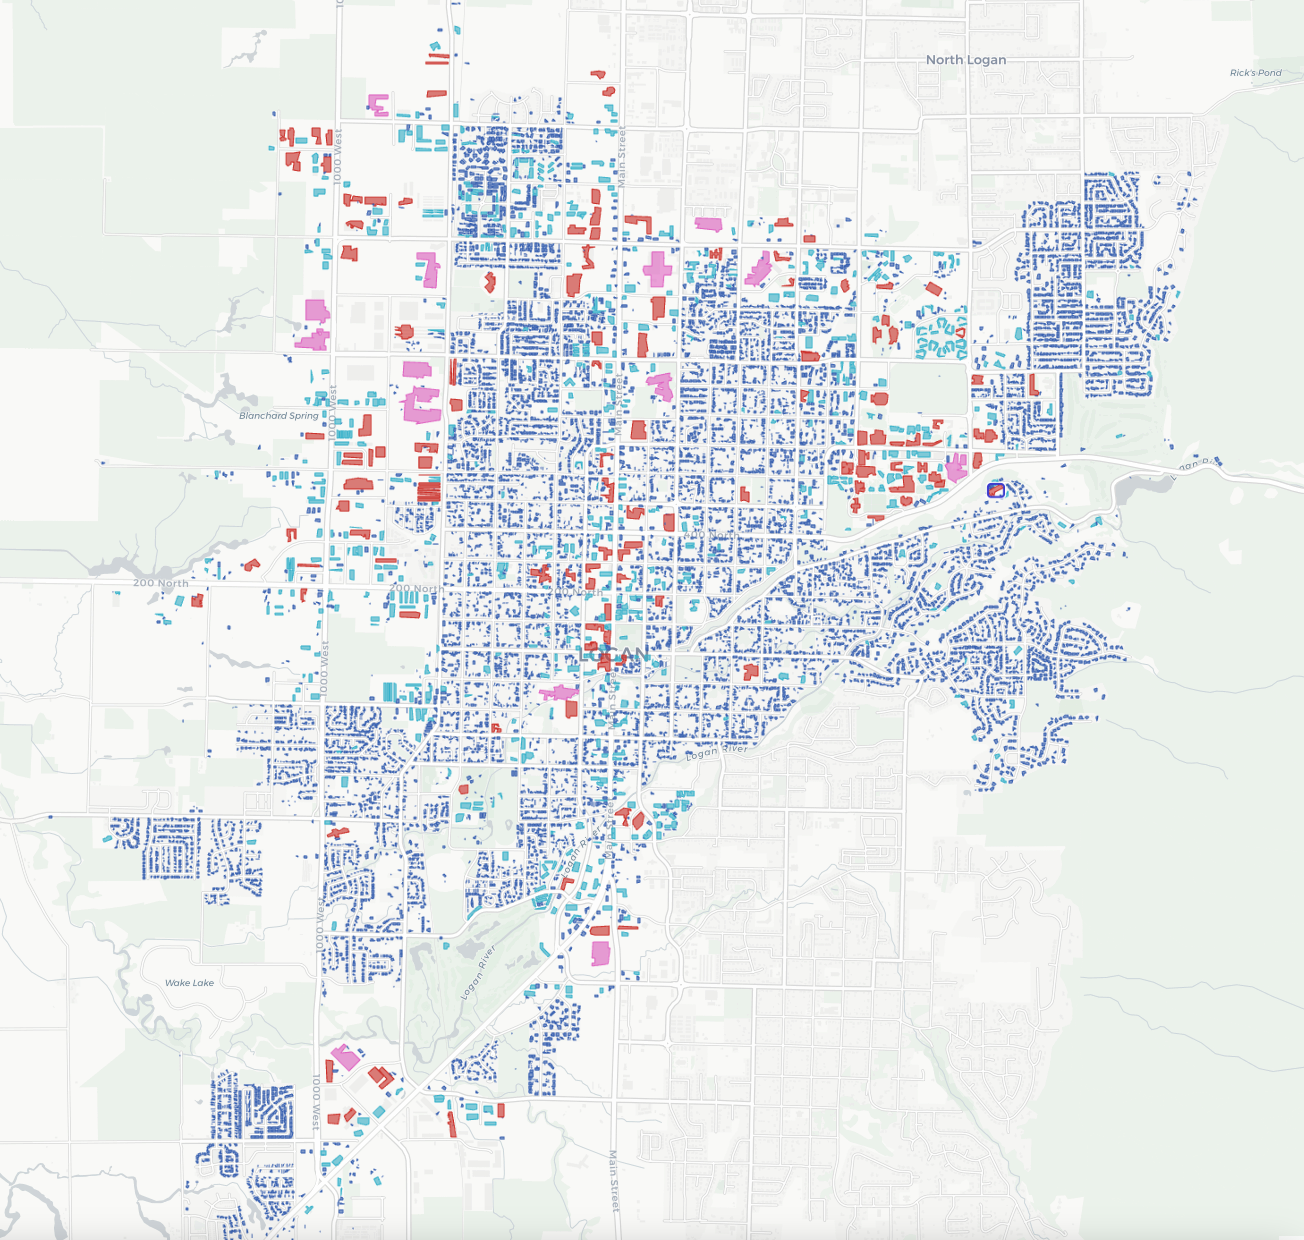
\includegraphics[width=1\linewidth,height=\textheight,keepaspectratio]{images_figures/building_footprints_logan.png}
\end{minipage}%
%
\begin{minipage}{0.50\linewidth}

\centering{

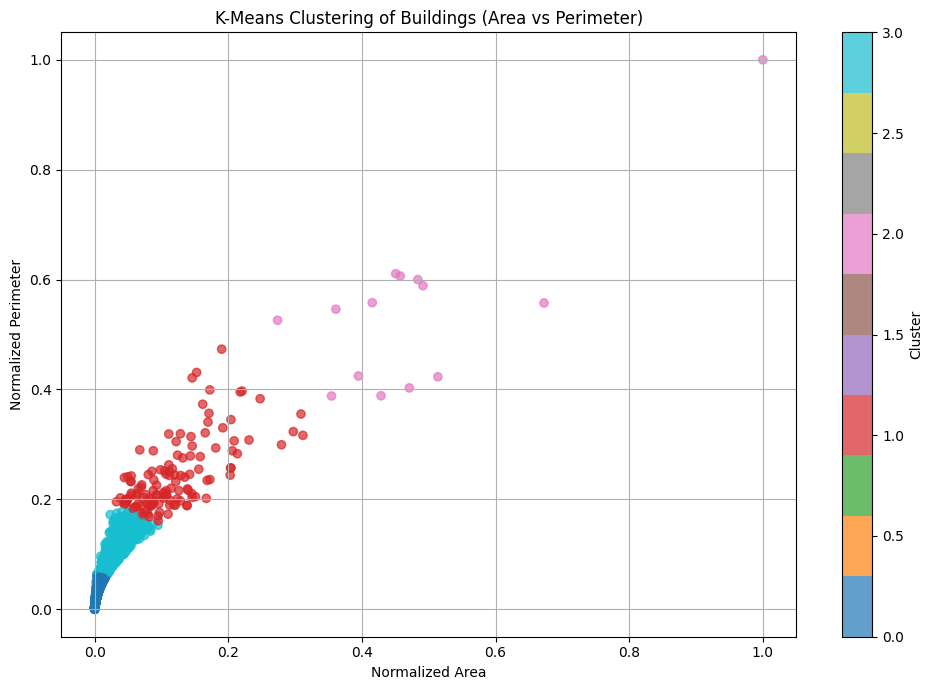
\includegraphics[width=1\linewidth,height=\textheight,keepaspectratio]{images_figures/Logan_Building_Cluster_plot_Normilized.png}

}

\subcaption{\label{fig-logan-bcp-n}Area vs parameter plot}

\end{minipage}%

\caption{\label{fig-logan-clusters-map-plot}K-mean analysis for Logan,
Utah}

\end{figure*}%

With the chosen city the latitude and longitude of the official city
boundries was obtained. Using this boundry, all the building footprints
in the city were extracted from the Microsoft Building Footprint dataset
and saved as a geojson file. The building were then classified using a
simple K-mean anaylsis to differentate different sized buildings. To do
this, the optimal K-mean was found using the elbow method. Using this K
vlaue, a K-mean anaysis was run comparing the areas of the building
footprints to their perimeters. Figure~\ref{fig-logan-clusters-map-plot}
shows the distribution of different cluster types, with most of the
buildings in Logan being a smaller size.

Using the building foorprint location and the python Library
``Contextily'', 600 randomly chosen aerial images of building in Logan
were taken from publicly availible satilite imagery and croped to focus
on a single building. 200 of the images were from clusters that included
only larger buildings to help balance building types in the dataset.

\subsection{Model Training}\label{model-training}

Ultraylitics' ``You Only Look Once'' or YOLO model is a open source
object detection model that has become very popular within do due it's
accuracy and ease of use. The model is trained on images that have been
previously annoatated, using bounding boxes, to identify the categories
desired for the model to detect. The model trains itself on these images
over many iterations until it is able to consistanly recongnize the
different categories of objects. The YOLO model is then able to predict
these categories in other images by bounding them in bounding boxes and
displaying the probability of correct identification.

Using the open source tool Label Studio, the collected street map images
were mannually annotated. This annotation including creating bounding
boxes around the roof of each buliding, using best judgement based off
the appearence of the building and surounding buildings and area. The
main buildings in each picture was labeld into five building categories:
Appartment, Residential, Commercial, Church, and School. This order was
consitant across annotations. These bounding boxes were saved as text
files and each one matched up with its corrisponding image.

The annotated data sets were split into two categories. 80\% of the
images were used in training the object dection model, while 20\% of the
images were reserved for validation purposes. Within these image sets
clusters that included larger and less common building sizes were
specifically included, due to thier relativily lower likelyhood of
appearing, to make sure the model would be trained on these less common
building types.

The model was run through hundreds of iterations until the model was
able to accuretly and reliably predict building types in Logan Utah. The
results of the final validation of the model is shown in
Figure~\ref{fig-confusion-matrix-logan}.

\begin{figure*}

\begin{minipage}{0.50\linewidth}

\centering{

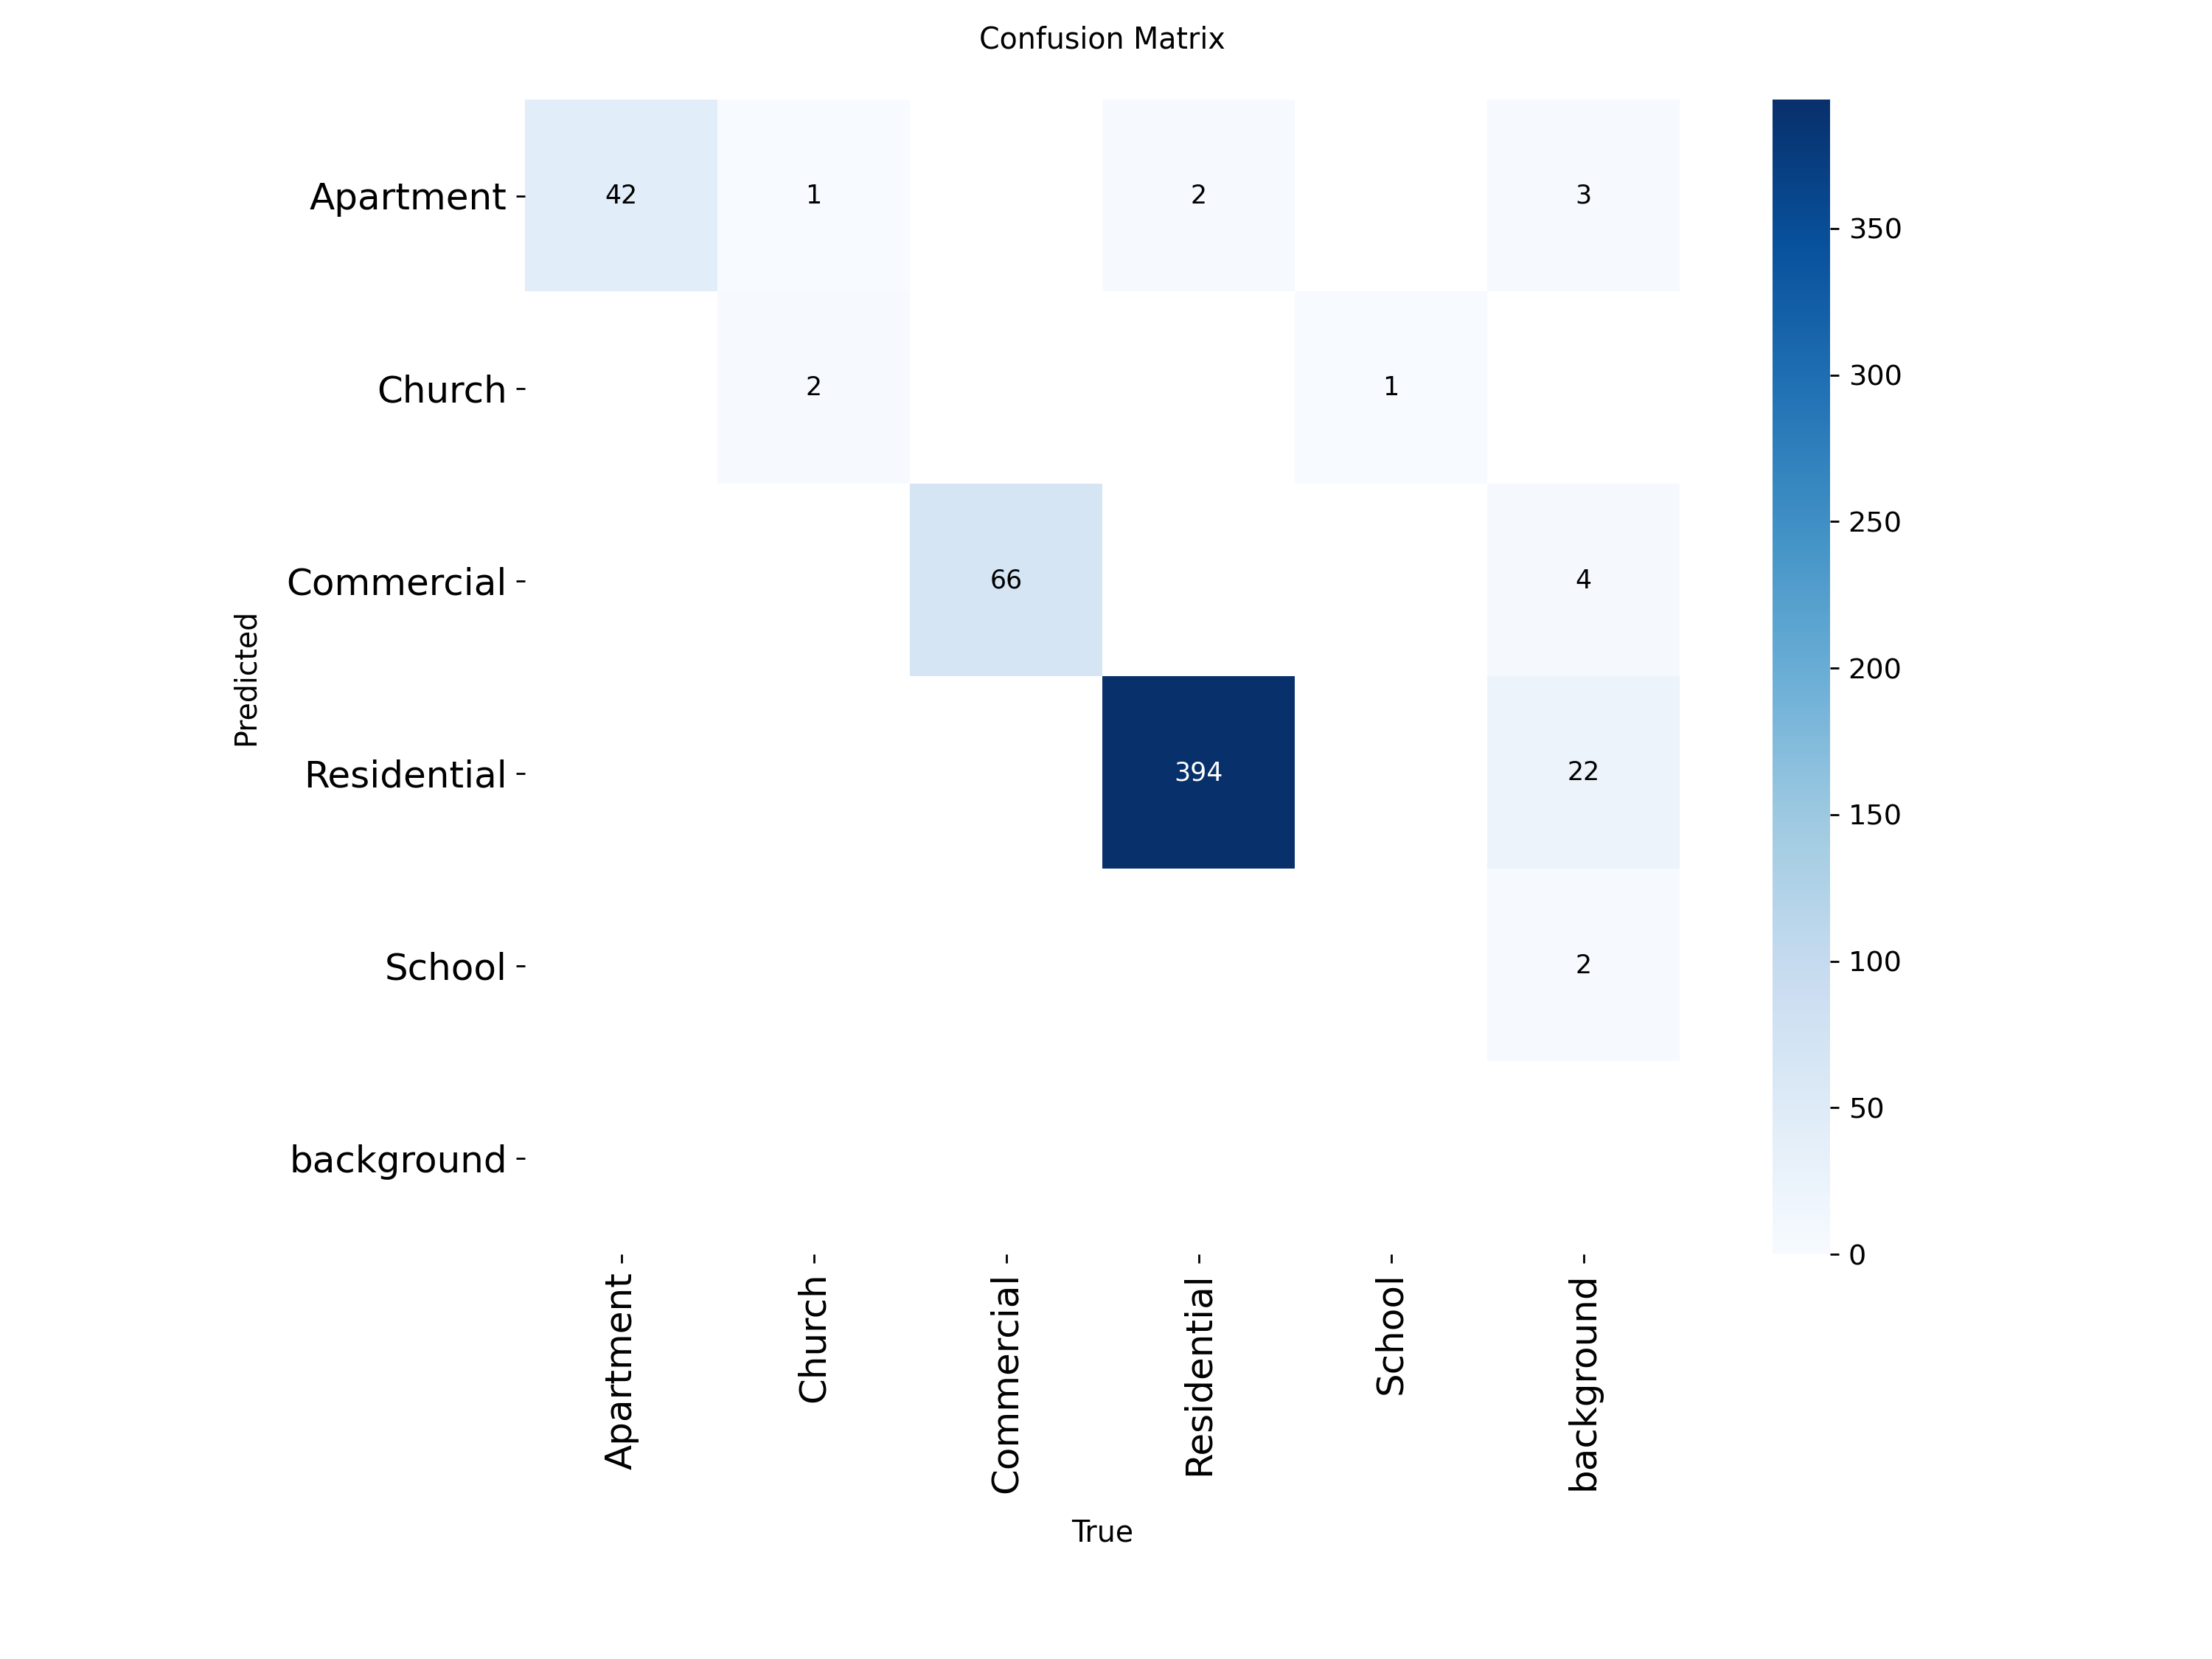
\includegraphics[width=1\linewidth,height=\textheight,keepaspectratio]{../runs/detect/logan_validation/confusion_matrix.png}

}

\subcaption{\label{fig-logan_cm}Logan confusion matrix}

\end{minipage}%
%
\begin{minipage}{0.50\linewidth}

\centering{

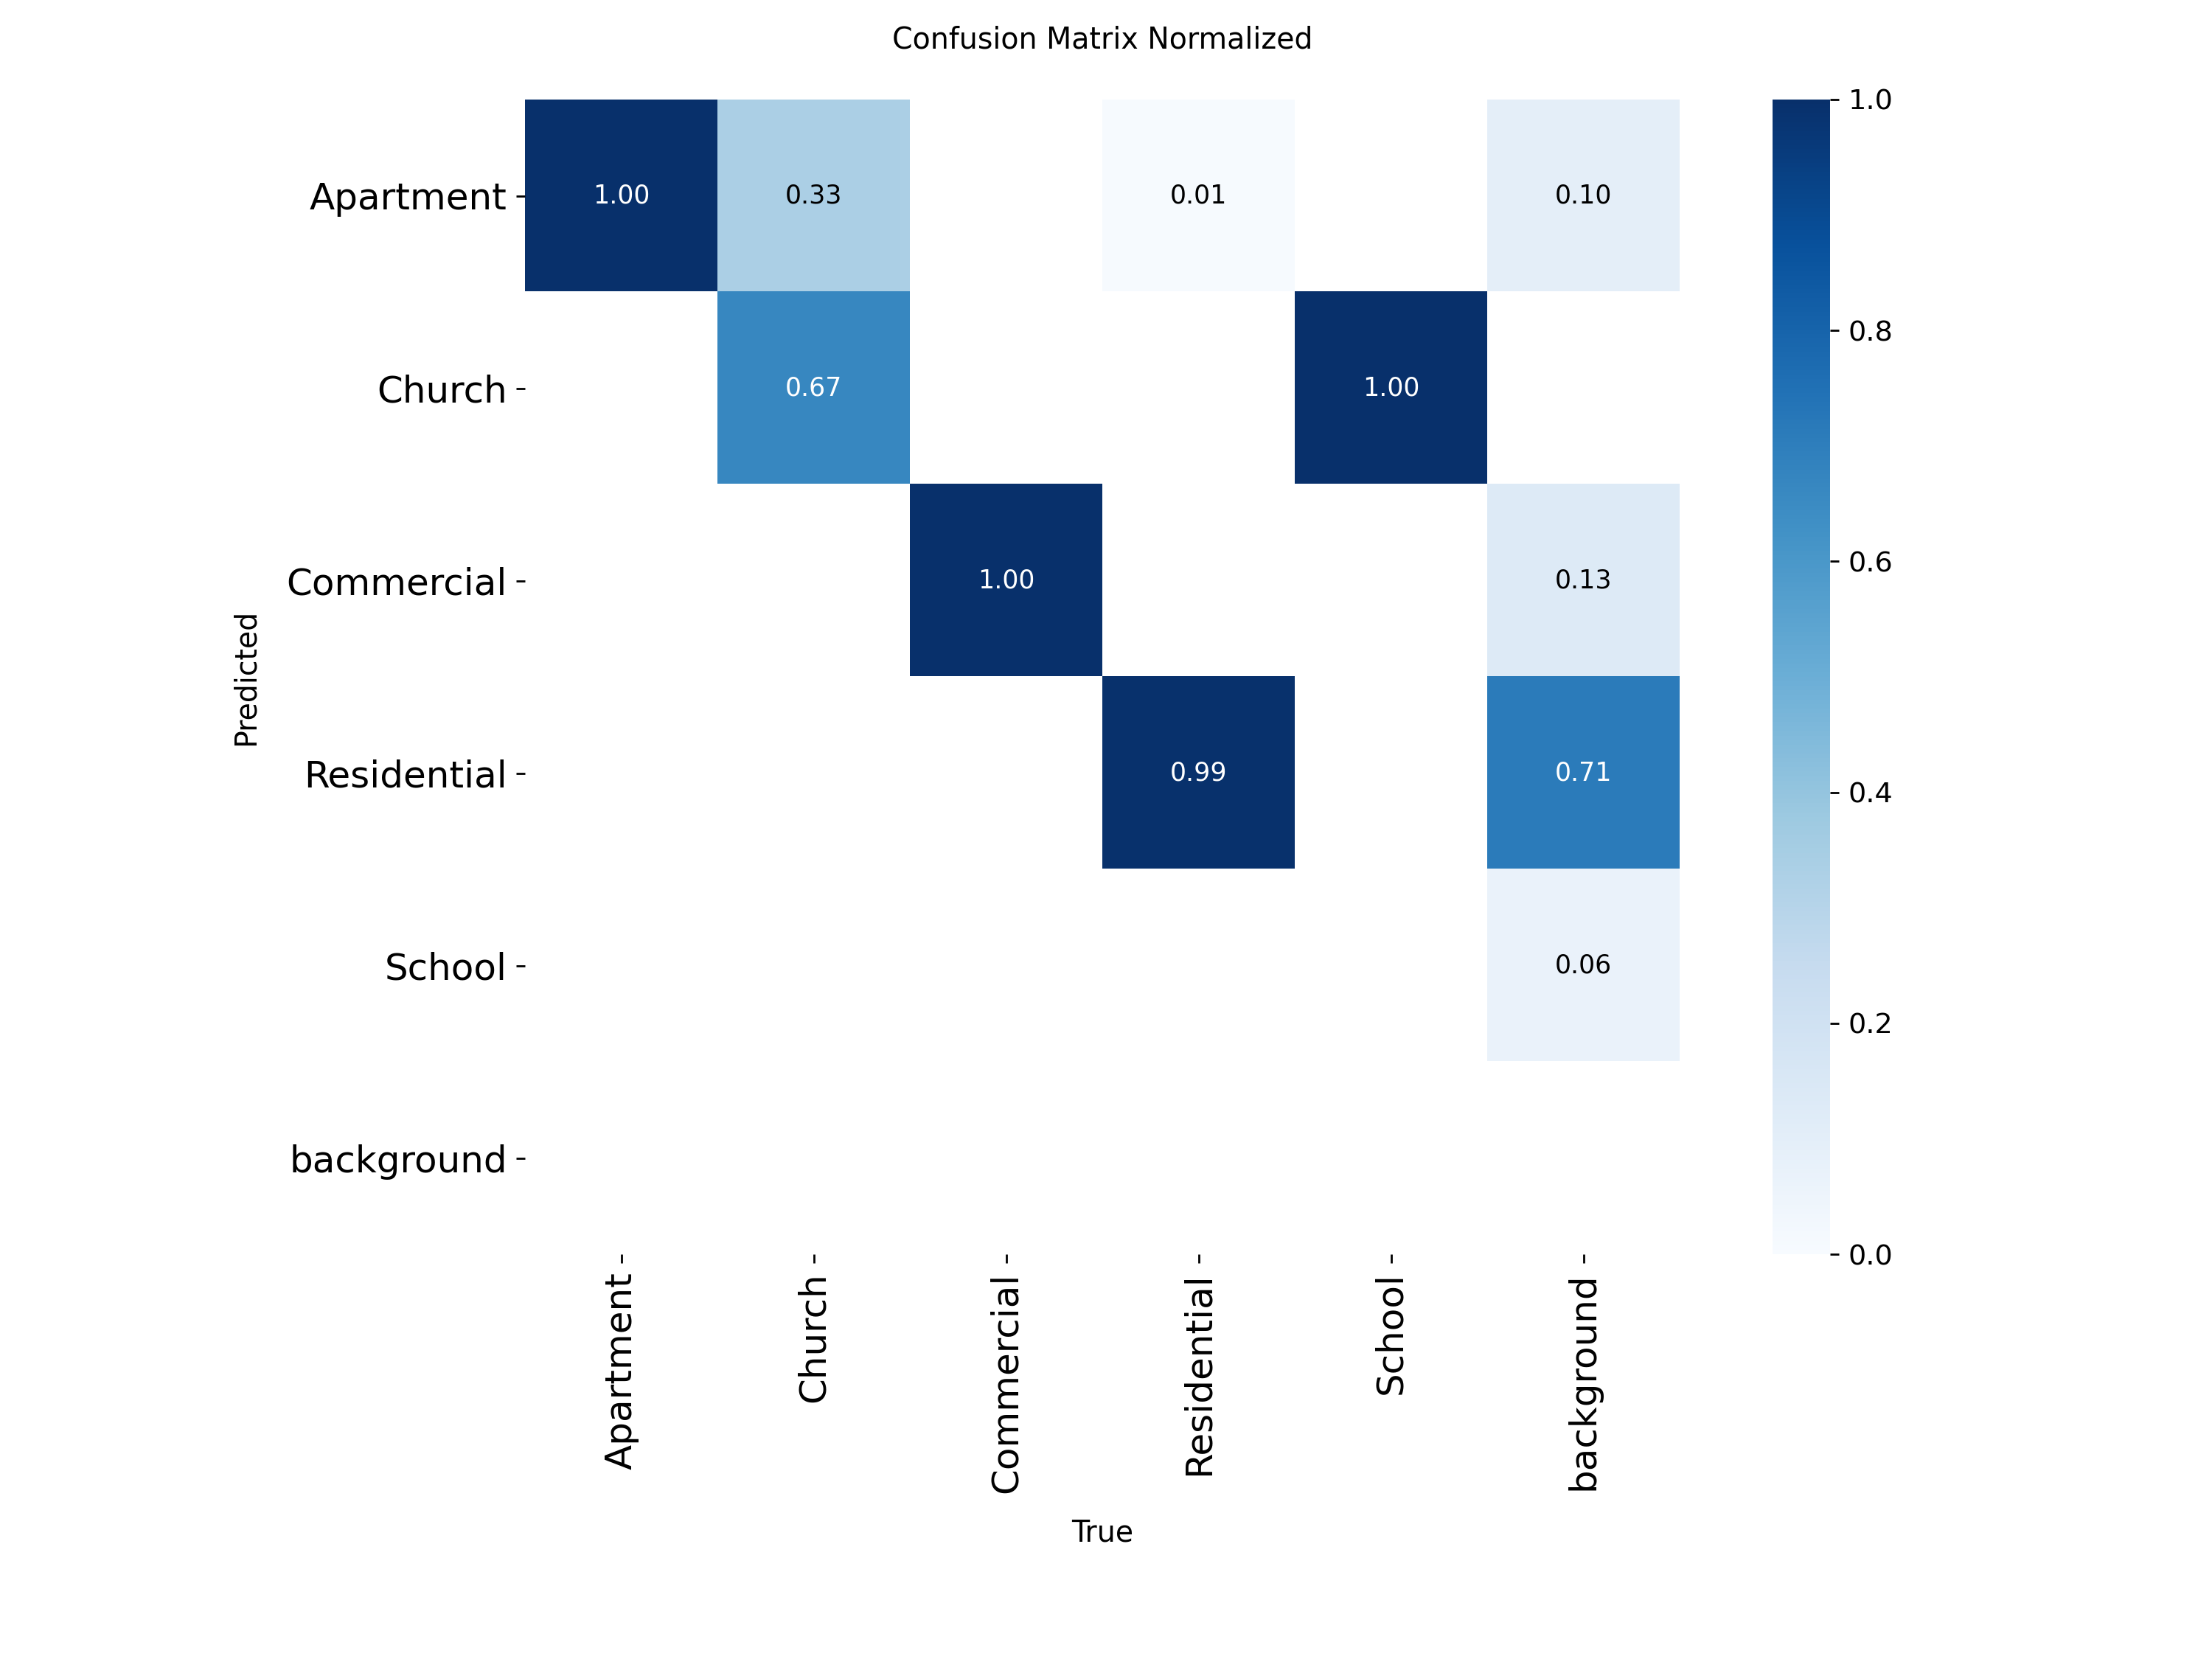
\includegraphics[width=1\linewidth,height=\textheight,keepaspectratio]{../runs/detect/logan_validation/confusion_matrix_normalized.png}

}

\subcaption{\label{fig-logan_cm_n}Logan confusion Matrix normalized}

\end{minipage}%

\caption{\label{fig-confusion-matrix-logan}YOLO confusion matrixes for
Logan, Utah.}

\end{figure*}%

\subsection{Model Validation and
Comparison}\label{model-validation-and-comparison}

Once the model was trained and validated using the Logan, Utah data set,
the model was then tested upon other cities in Utah to assess it's
viablity in predicting building categories elsewhere in Utah. Using
American Community Survey data, five other test cities were chosen based
off the city's median income level, and the median age of the homes. The
chosen cities an been seen in Table~\ref{tbl-val-cities}.

\begin{table}

\caption{\label{tbl-val-cities}}

\centering{

\subcaption{\label{tbl-val-cities}Chosen Cities Based off Median Income and House Age}

\centering{

\centering


\renewcommand{\arraystretch}{1.3}
\begin{tabular}{lccccc}
\hline
House Age & High Income & Middle Income & Low Income  \\
\hline
Old Houses   & Bountiful, Utah    & Ogden, Utah        & Price, Utah         \\
New Houses & Saratoga Springs    & St. George, Utah         & (None)         \\
\hline
\end{tabular}

}

}

\end{table}%

Following the same method as previously described, building footrpint
data was collected and analized for each city. 200 aerial images of
buildings were randomly chosen and annotated. These annotated data sets
were then run through the model using validation only. The results of
these runs are given below in
Figure~\ref{fig-confusion-matrix-val-cities}. These results were then
analyses to evaluate the ability of the model to predict in other
cities, as well as assess if household income or house age were
indicating factors.

\section{Results and Discussion}\label{results-and-discussion}

The Logan trained YOLO model was able to accurantly predicit
residnetial, commercial, and apartment building types almost 100\% of
the time, as shown in Figure~\ref{fig-confusion-matrix-logan}. The
desired outcome is to have all the numbers in a diagonal line, which
would indicate that the model is predicting the category of a building
that is in line with the annotations made.

The model did underpreform wich schools and churches. This is attributed
to the fact that there were very low number of images of both building
types provided during model training.

A important aspect to discuss is the model predicitng different building
types where there is no building. This is seen on the far right of each
graph, where the background was categorized. This error occurs from two
sources. One is the annotation. Building such as backyard sheds were not
identified, but the model still picked them up. Or there were times that
only a fouth of a building was present in an image, and so was not
annotated, but was still recongized by the model at a lower probability
level. The other source of error is the quality of the photos used. The
satilite images from Contextily were convient and easy to access, but
were not high quality. This resulted in the model sometimes interpreting
things of solid colors, such as roads and covered parking as a type of
building. The second error could be solved using higher quality photos,
while the first

Confusion matrix for other analysis cities. What is the results? Was
there a difference between how the model did between the cities? Was age
of the house a big factor? Was income? Is there something else? Neither
house age or house median income made a difference in the calssification
of houses.

Given the results of the validations, a process to develop a model for
different locations would be more useful and viable then to create a
universal model used in a wide area.

However, much of this research is supseptible to similar probelems as
transporation models. Satilite remote sensing data is not consistent
around the world, having varying availibiilyt and image quality.

\begin{figure*}

\begin{minipage}{0.50\linewidth}

\centering{

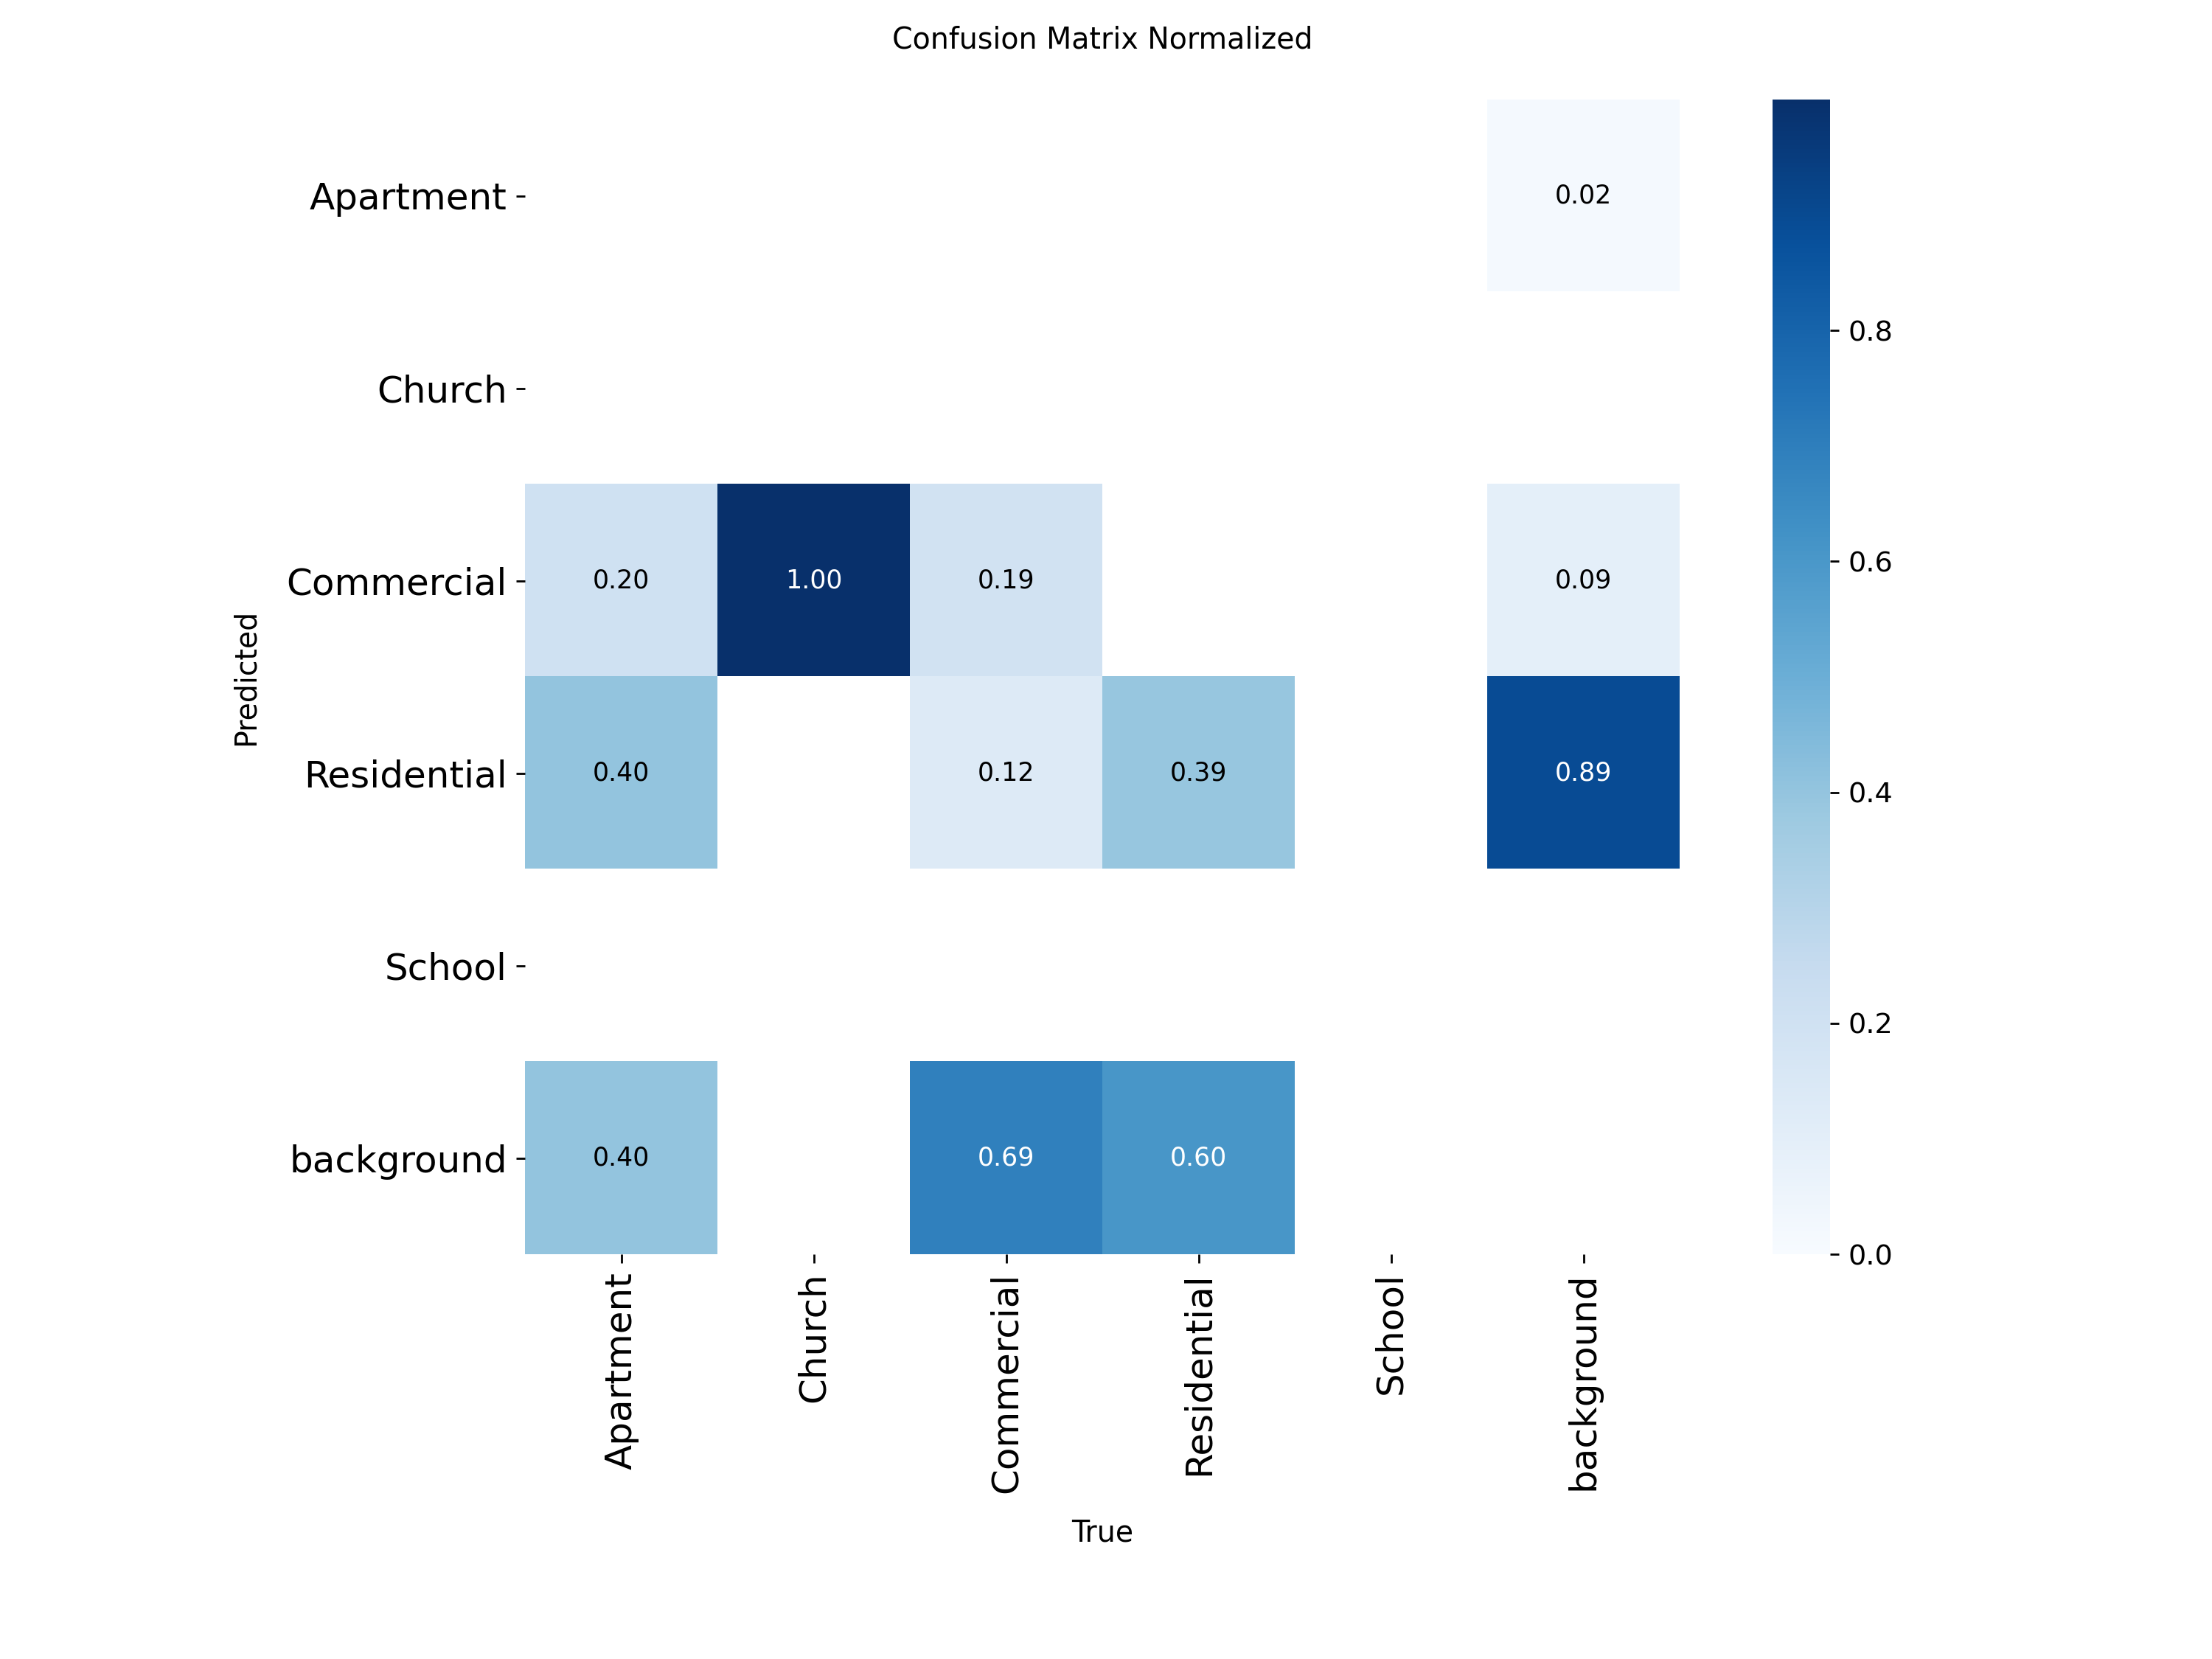
\includegraphics[width=1\linewidth,height=\textheight,keepaspectratio]{../runs/detect/bountiful_validation/confusion_matrix_normalized.png}

}

\subcaption{\label{fig-logan_cm}Bountiful, Utah}

\end{minipage}%
%
\begin{minipage}{0.50\linewidth}

\centering{

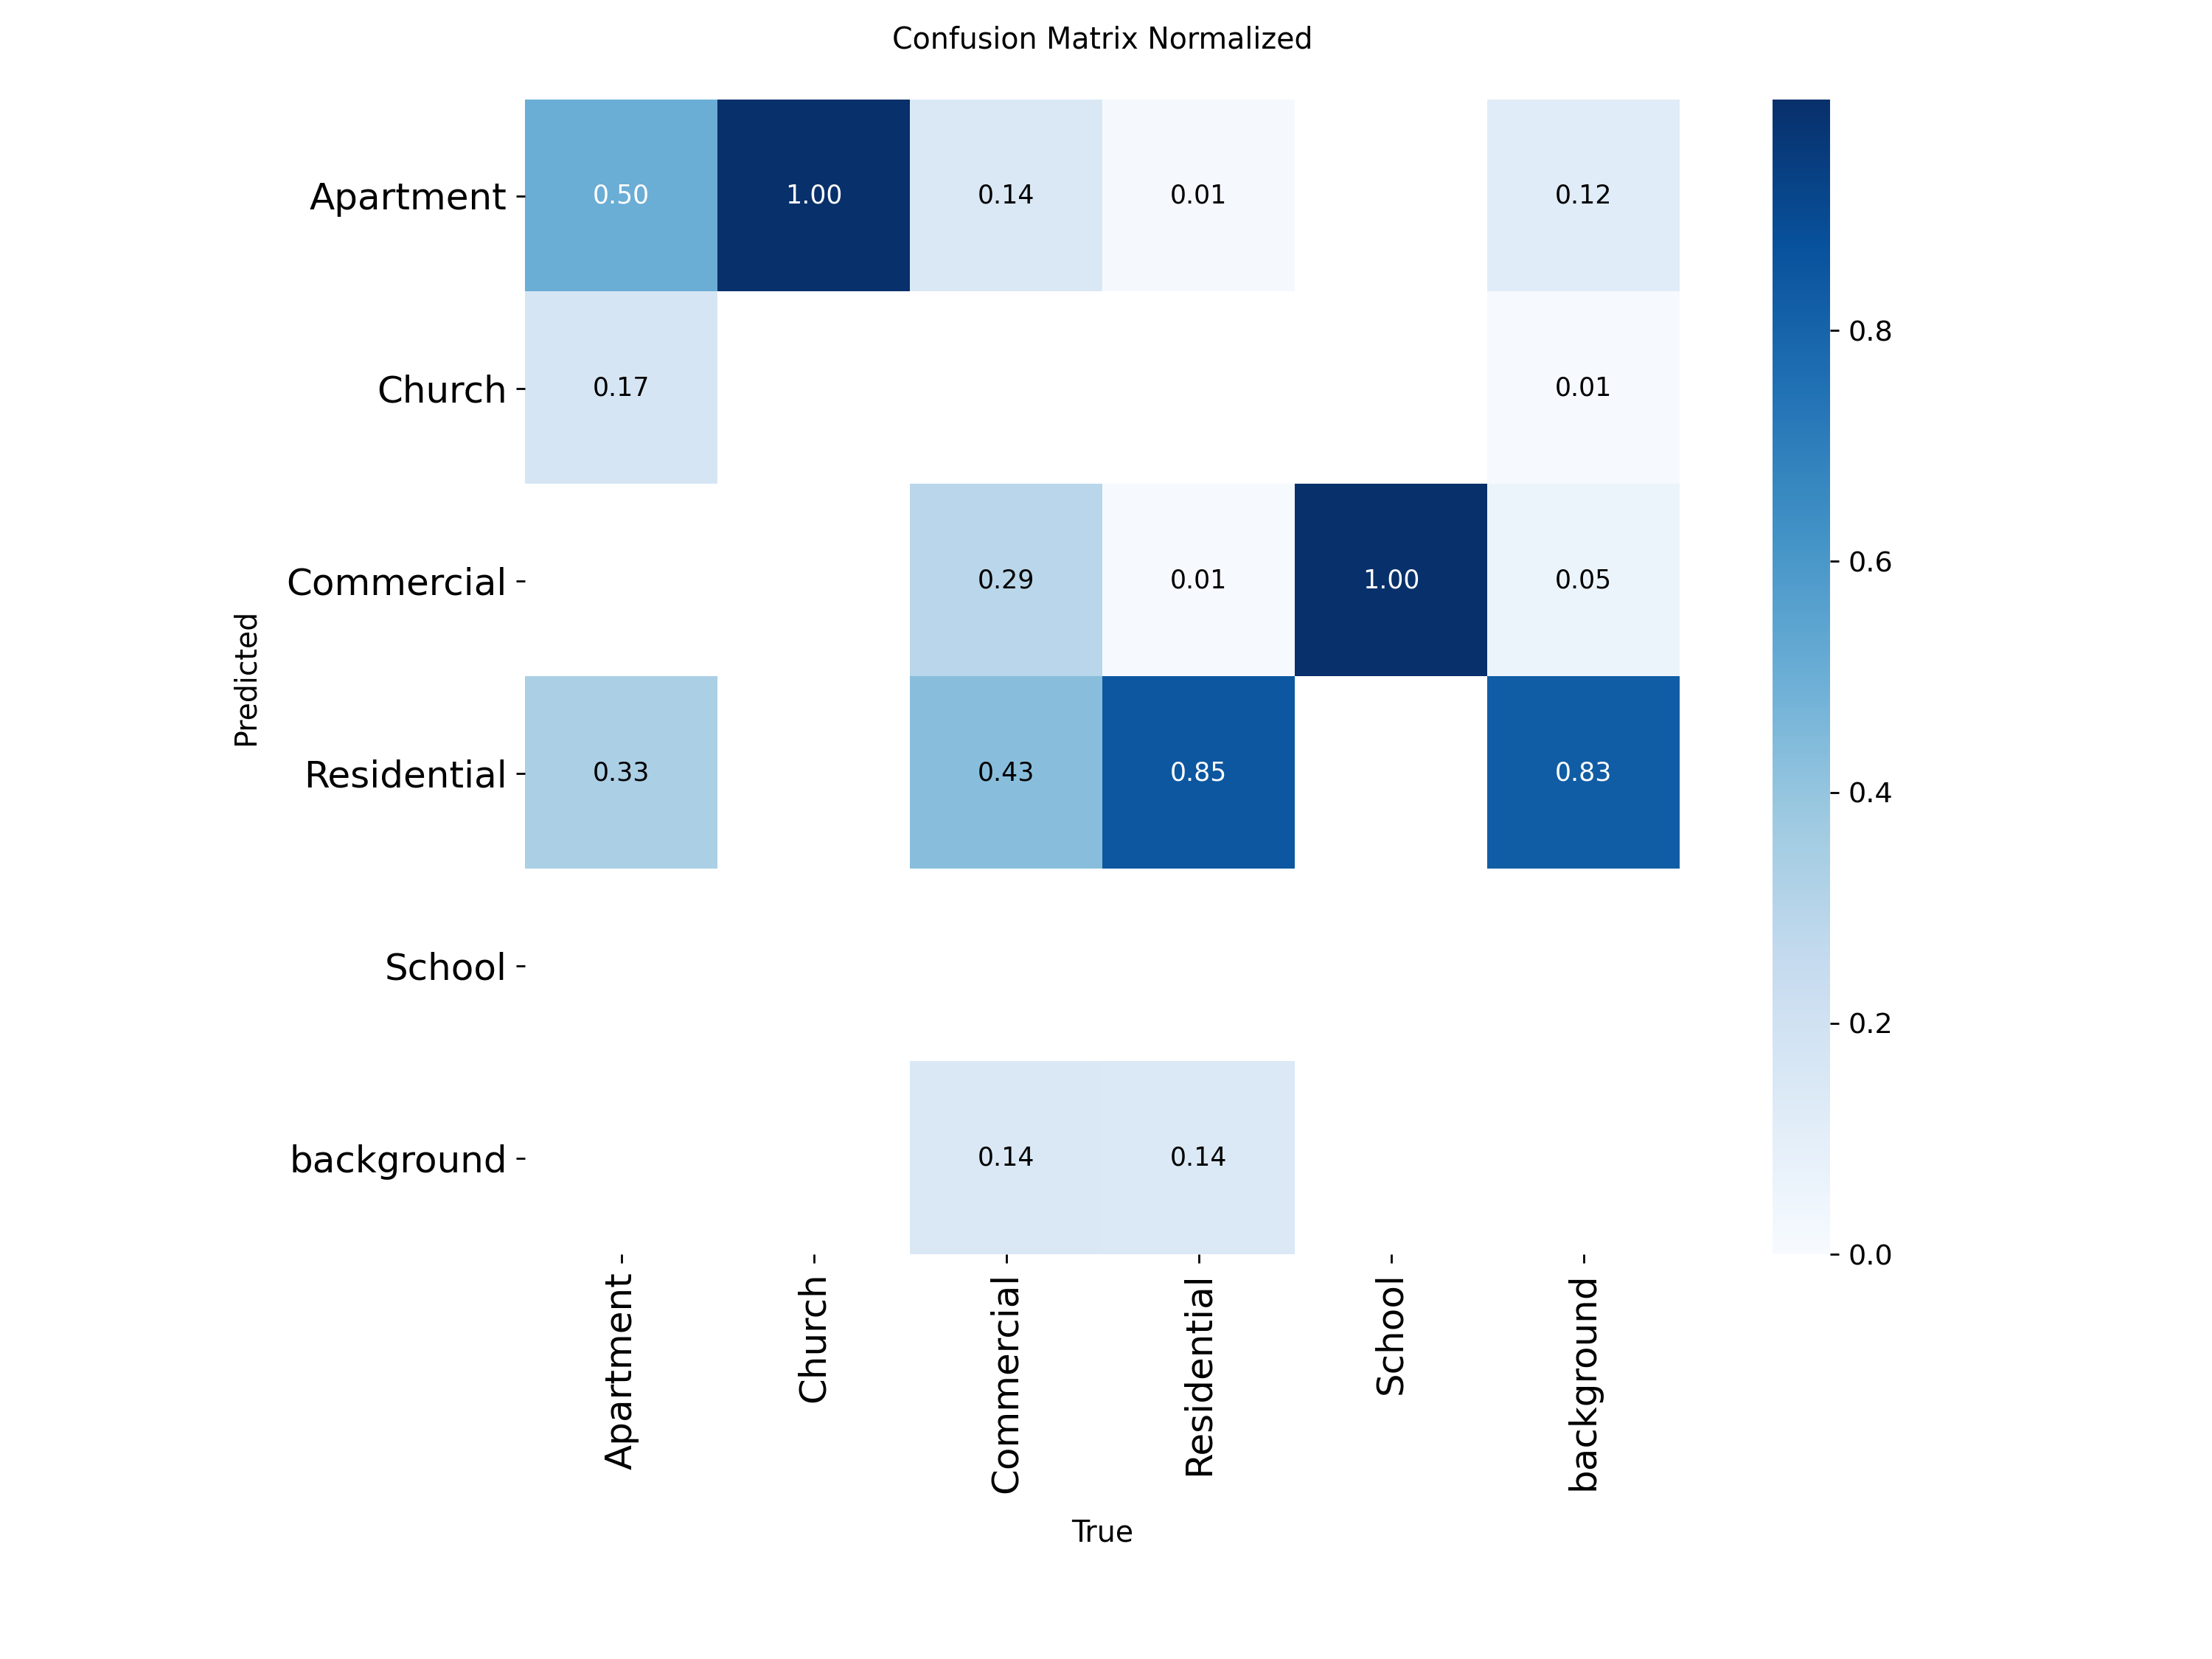
\includegraphics[width=1\linewidth,height=\textheight,keepaspectratio]{../runs/detect/saratoga_springs_validation/confusion_matrix_normalized.png}

}

\subcaption{\label{fig-logan_cm_n}Saratoga Springs, Utah}

\end{minipage}%
\newline
\begin{minipage}{0.50\linewidth}

\centering{

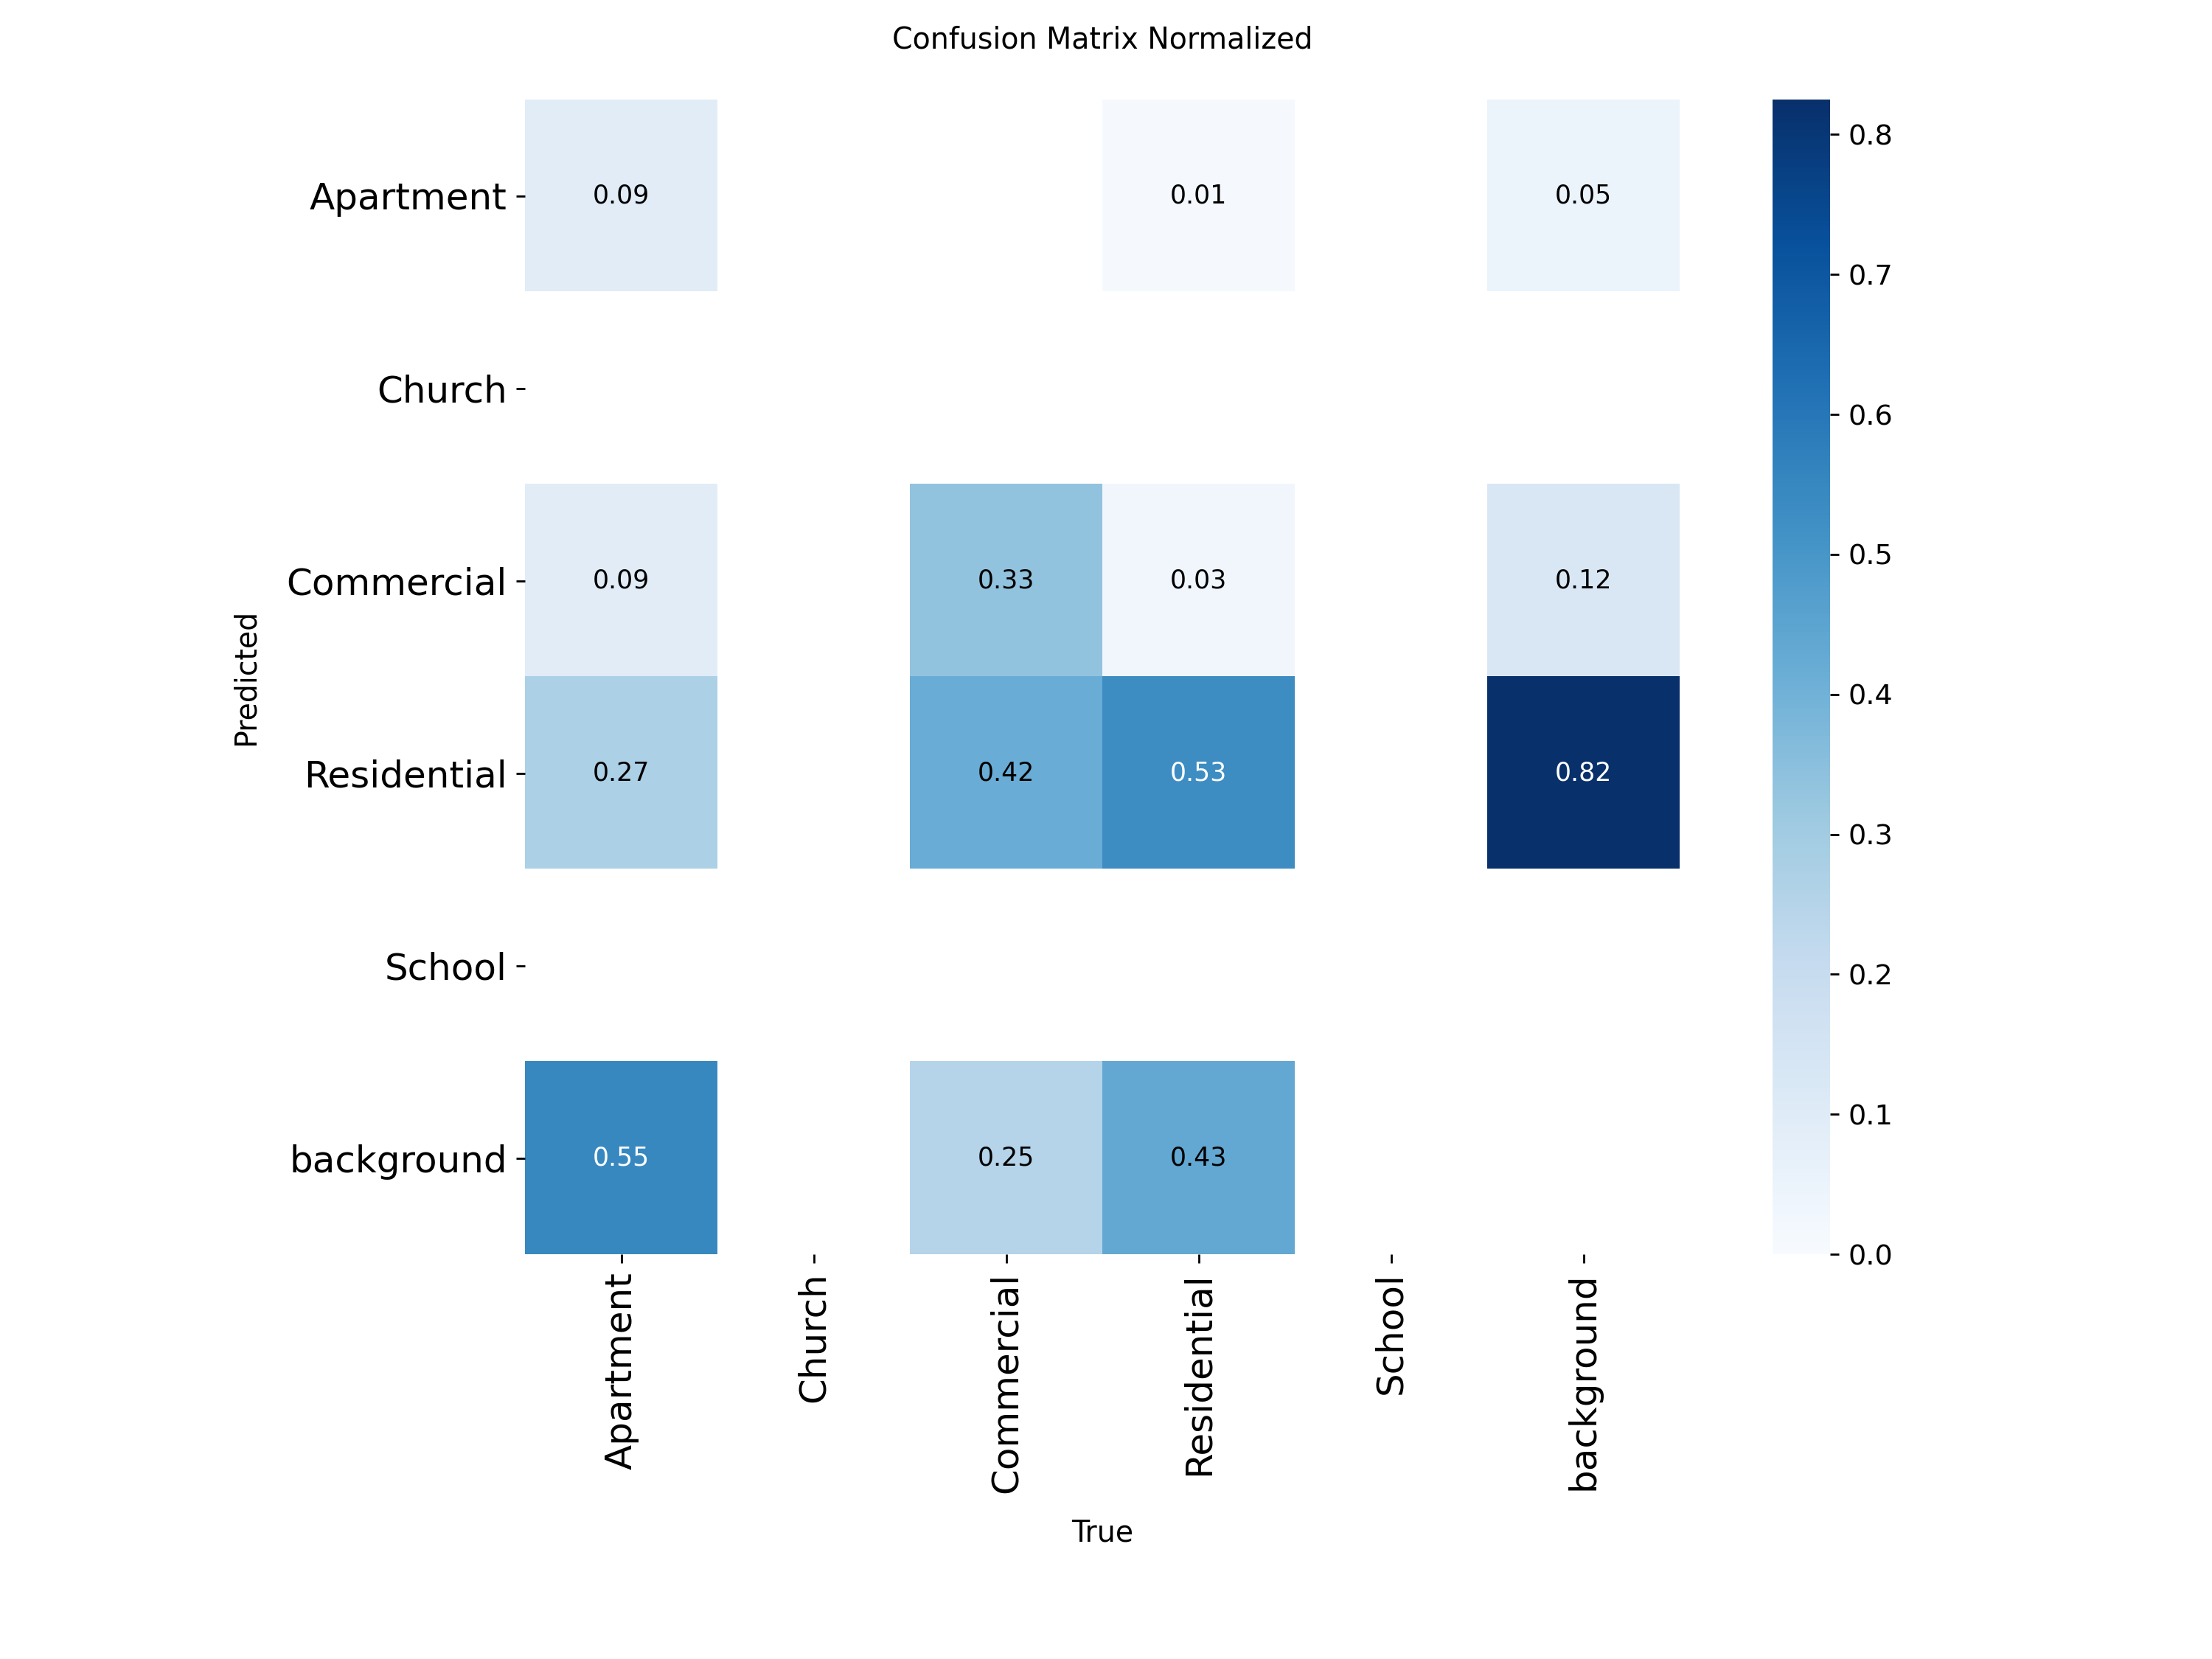
\includegraphics[width=1\linewidth,height=\textheight,keepaspectratio]{../runs/detect/ogden_validation/confusion_matrix_normalized.png}

}

\subcaption{\label{fig-logan_cm}Ogden, Utah}

\end{minipage}%
%
\begin{minipage}{0.50\linewidth}

\centering{

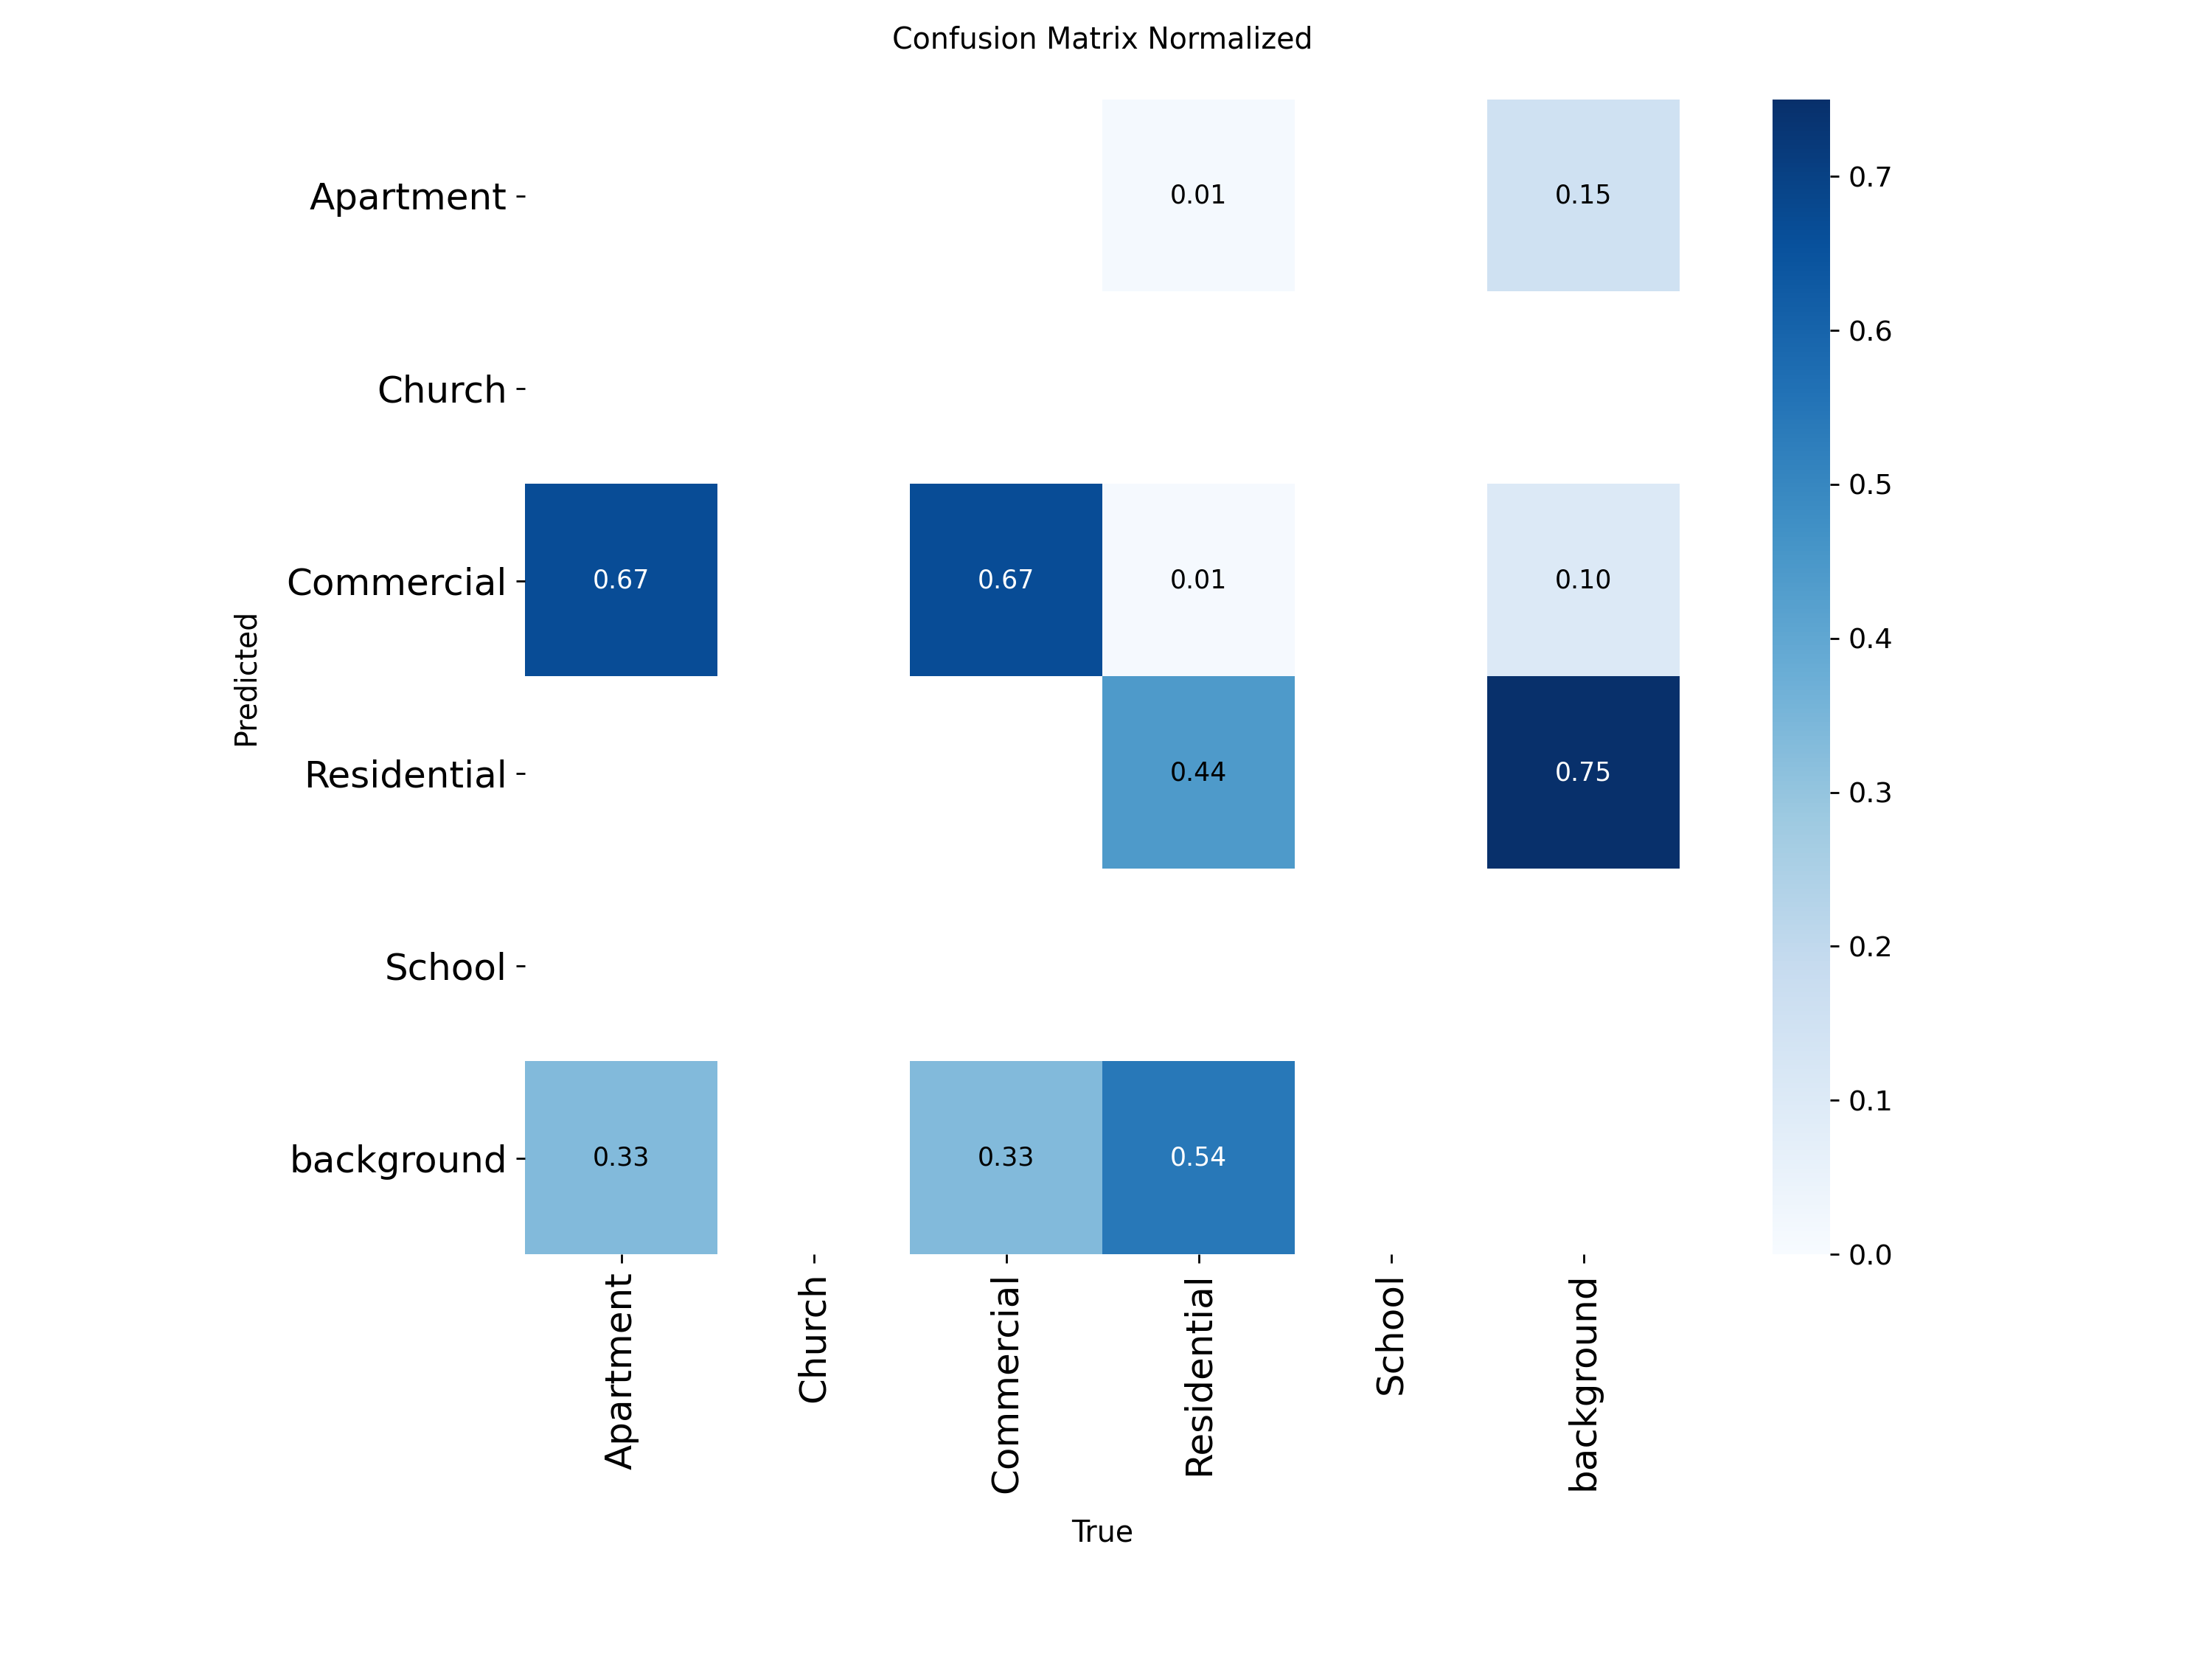
\includegraphics[width=1\linewidth,height=\textheight,keepaspectratio]{../runs/detect/st_george_validation/confusion_matrix_normalized.png}

}

\subcaption{\label{fig-logan_cm_n}St.~George, Utah}

\end{minipage}%
\newline
\begin{minipage}{0.50\linewidth}

\centering{

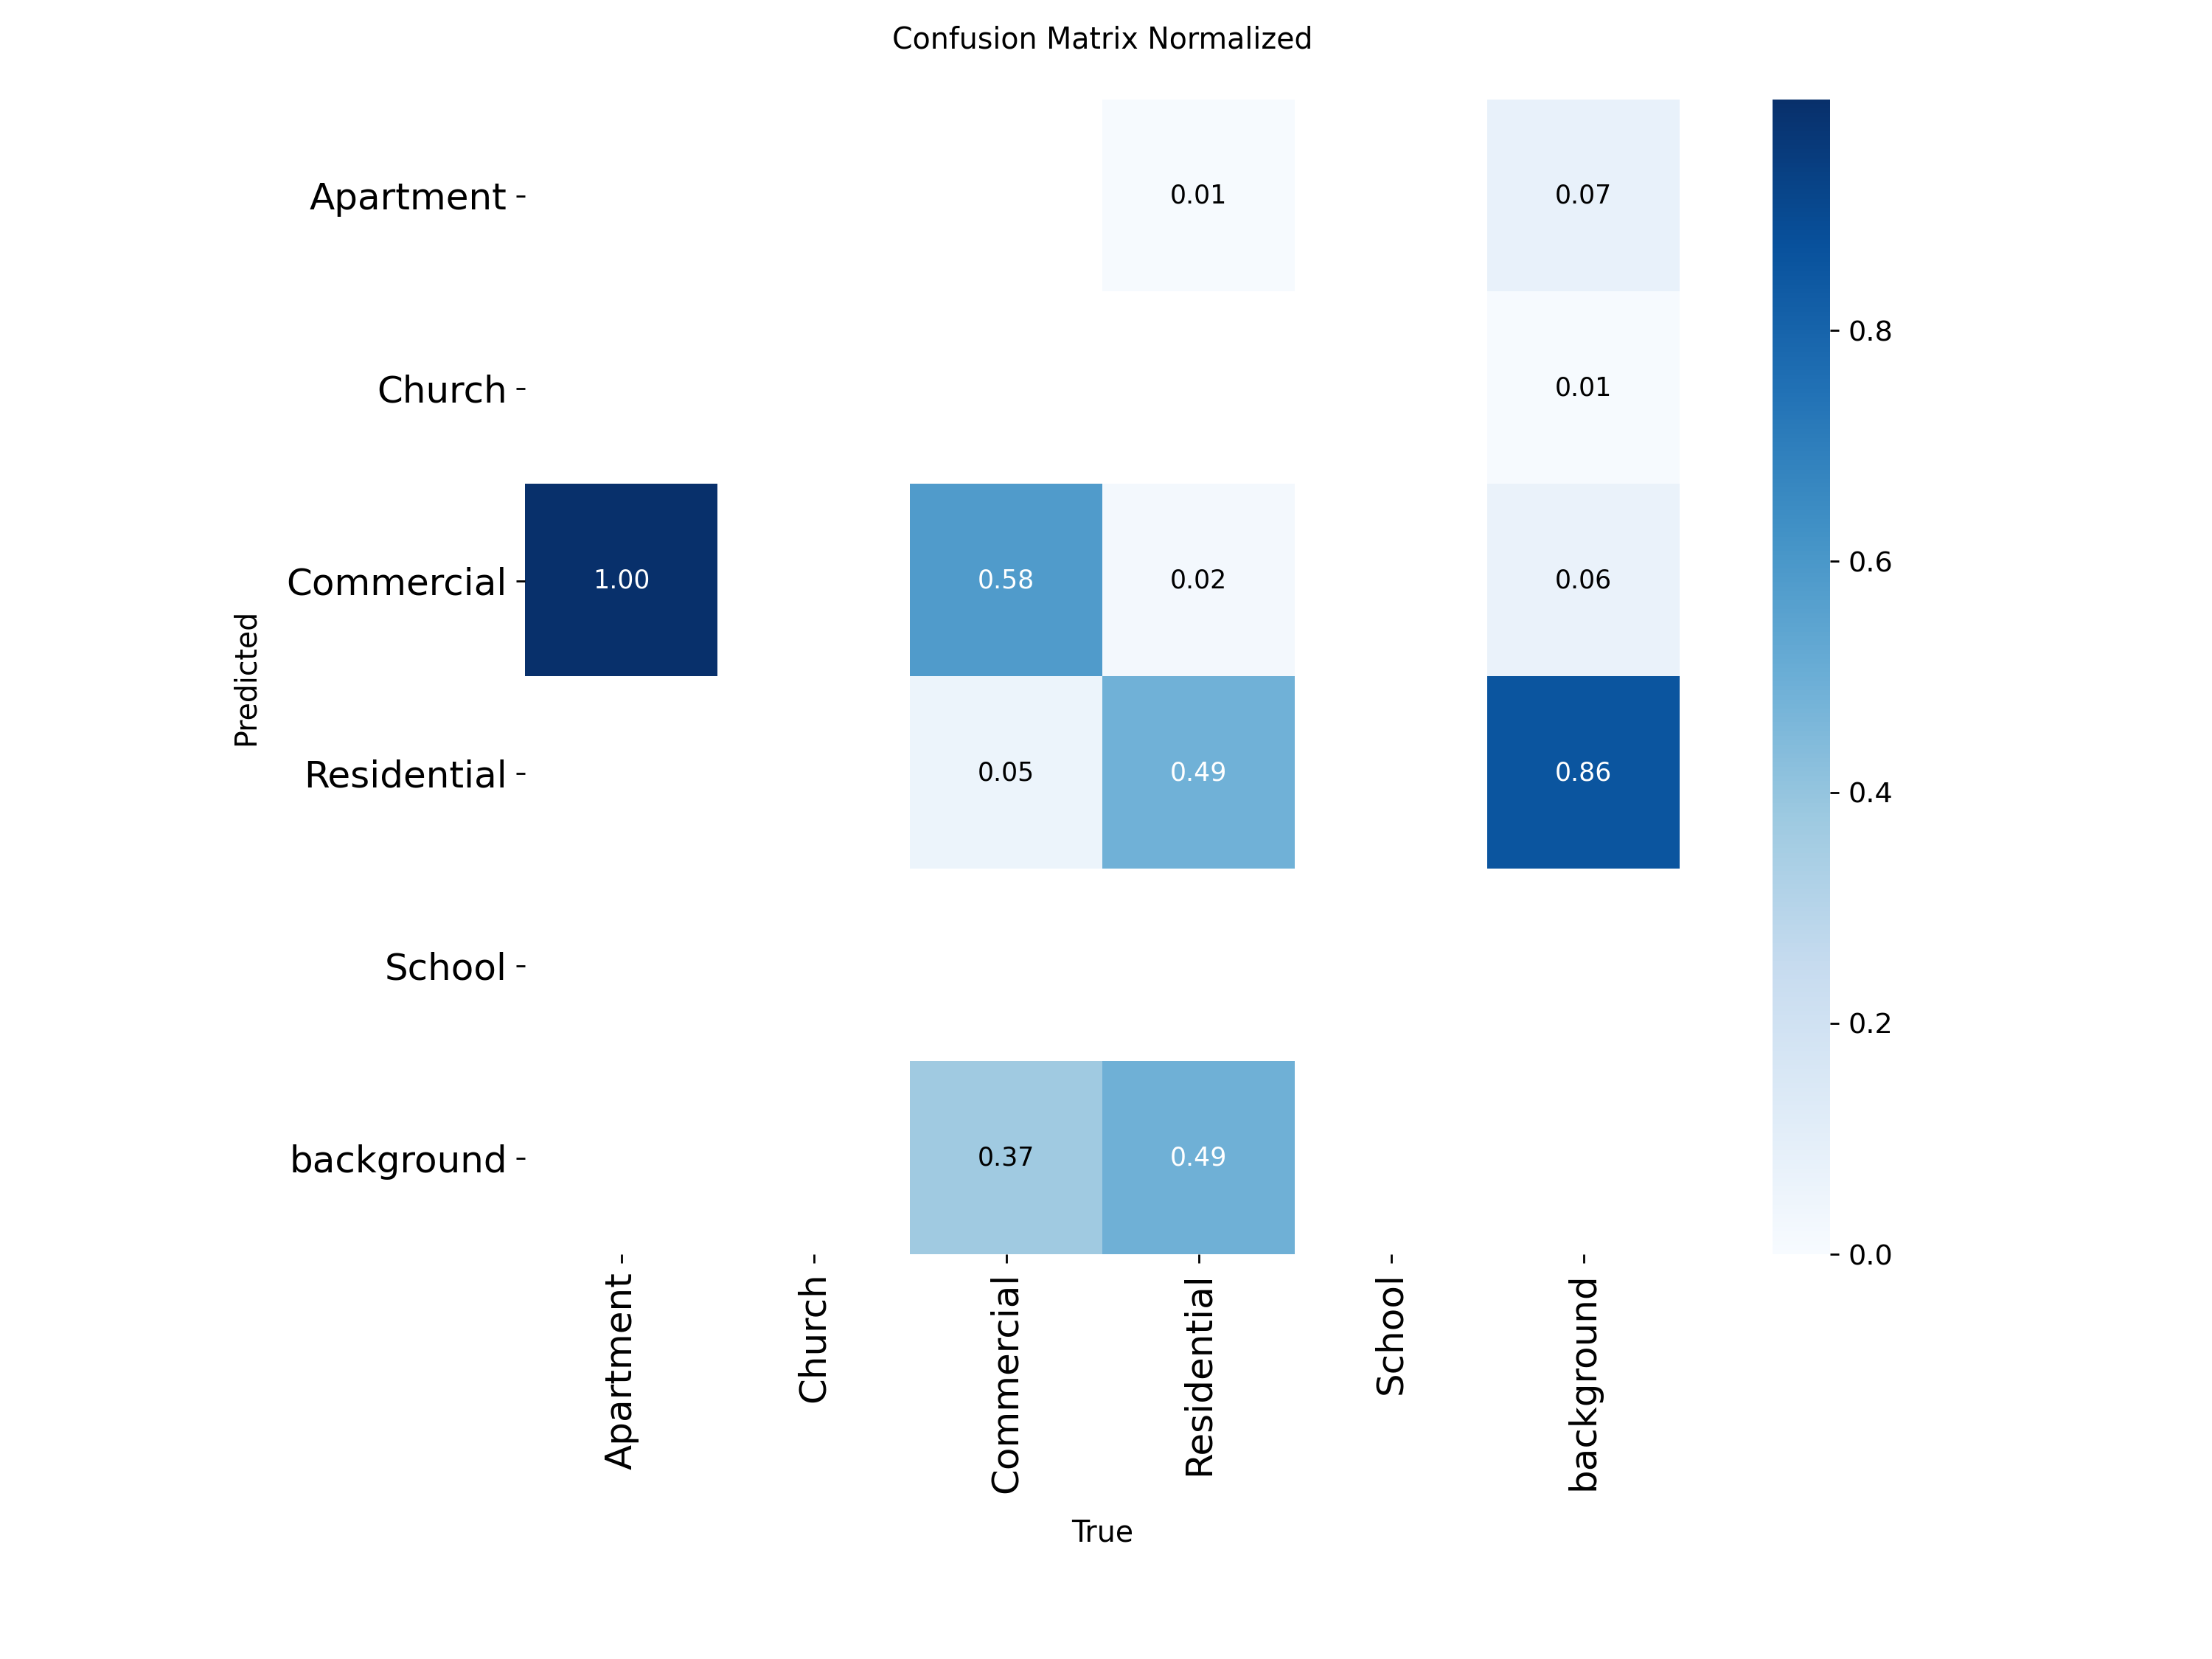
\includegraphics[width=1\linewidth,height=\textheight,keepaspectratio]{../runs/detect/price_validation/confusion_matrix_normalized.png}

}

\subcaption{\label{fig-logan_cm}Price, Utah}

\end{minipage}%
%
\begin{minipage}{0.50\linewidth}

\centering{

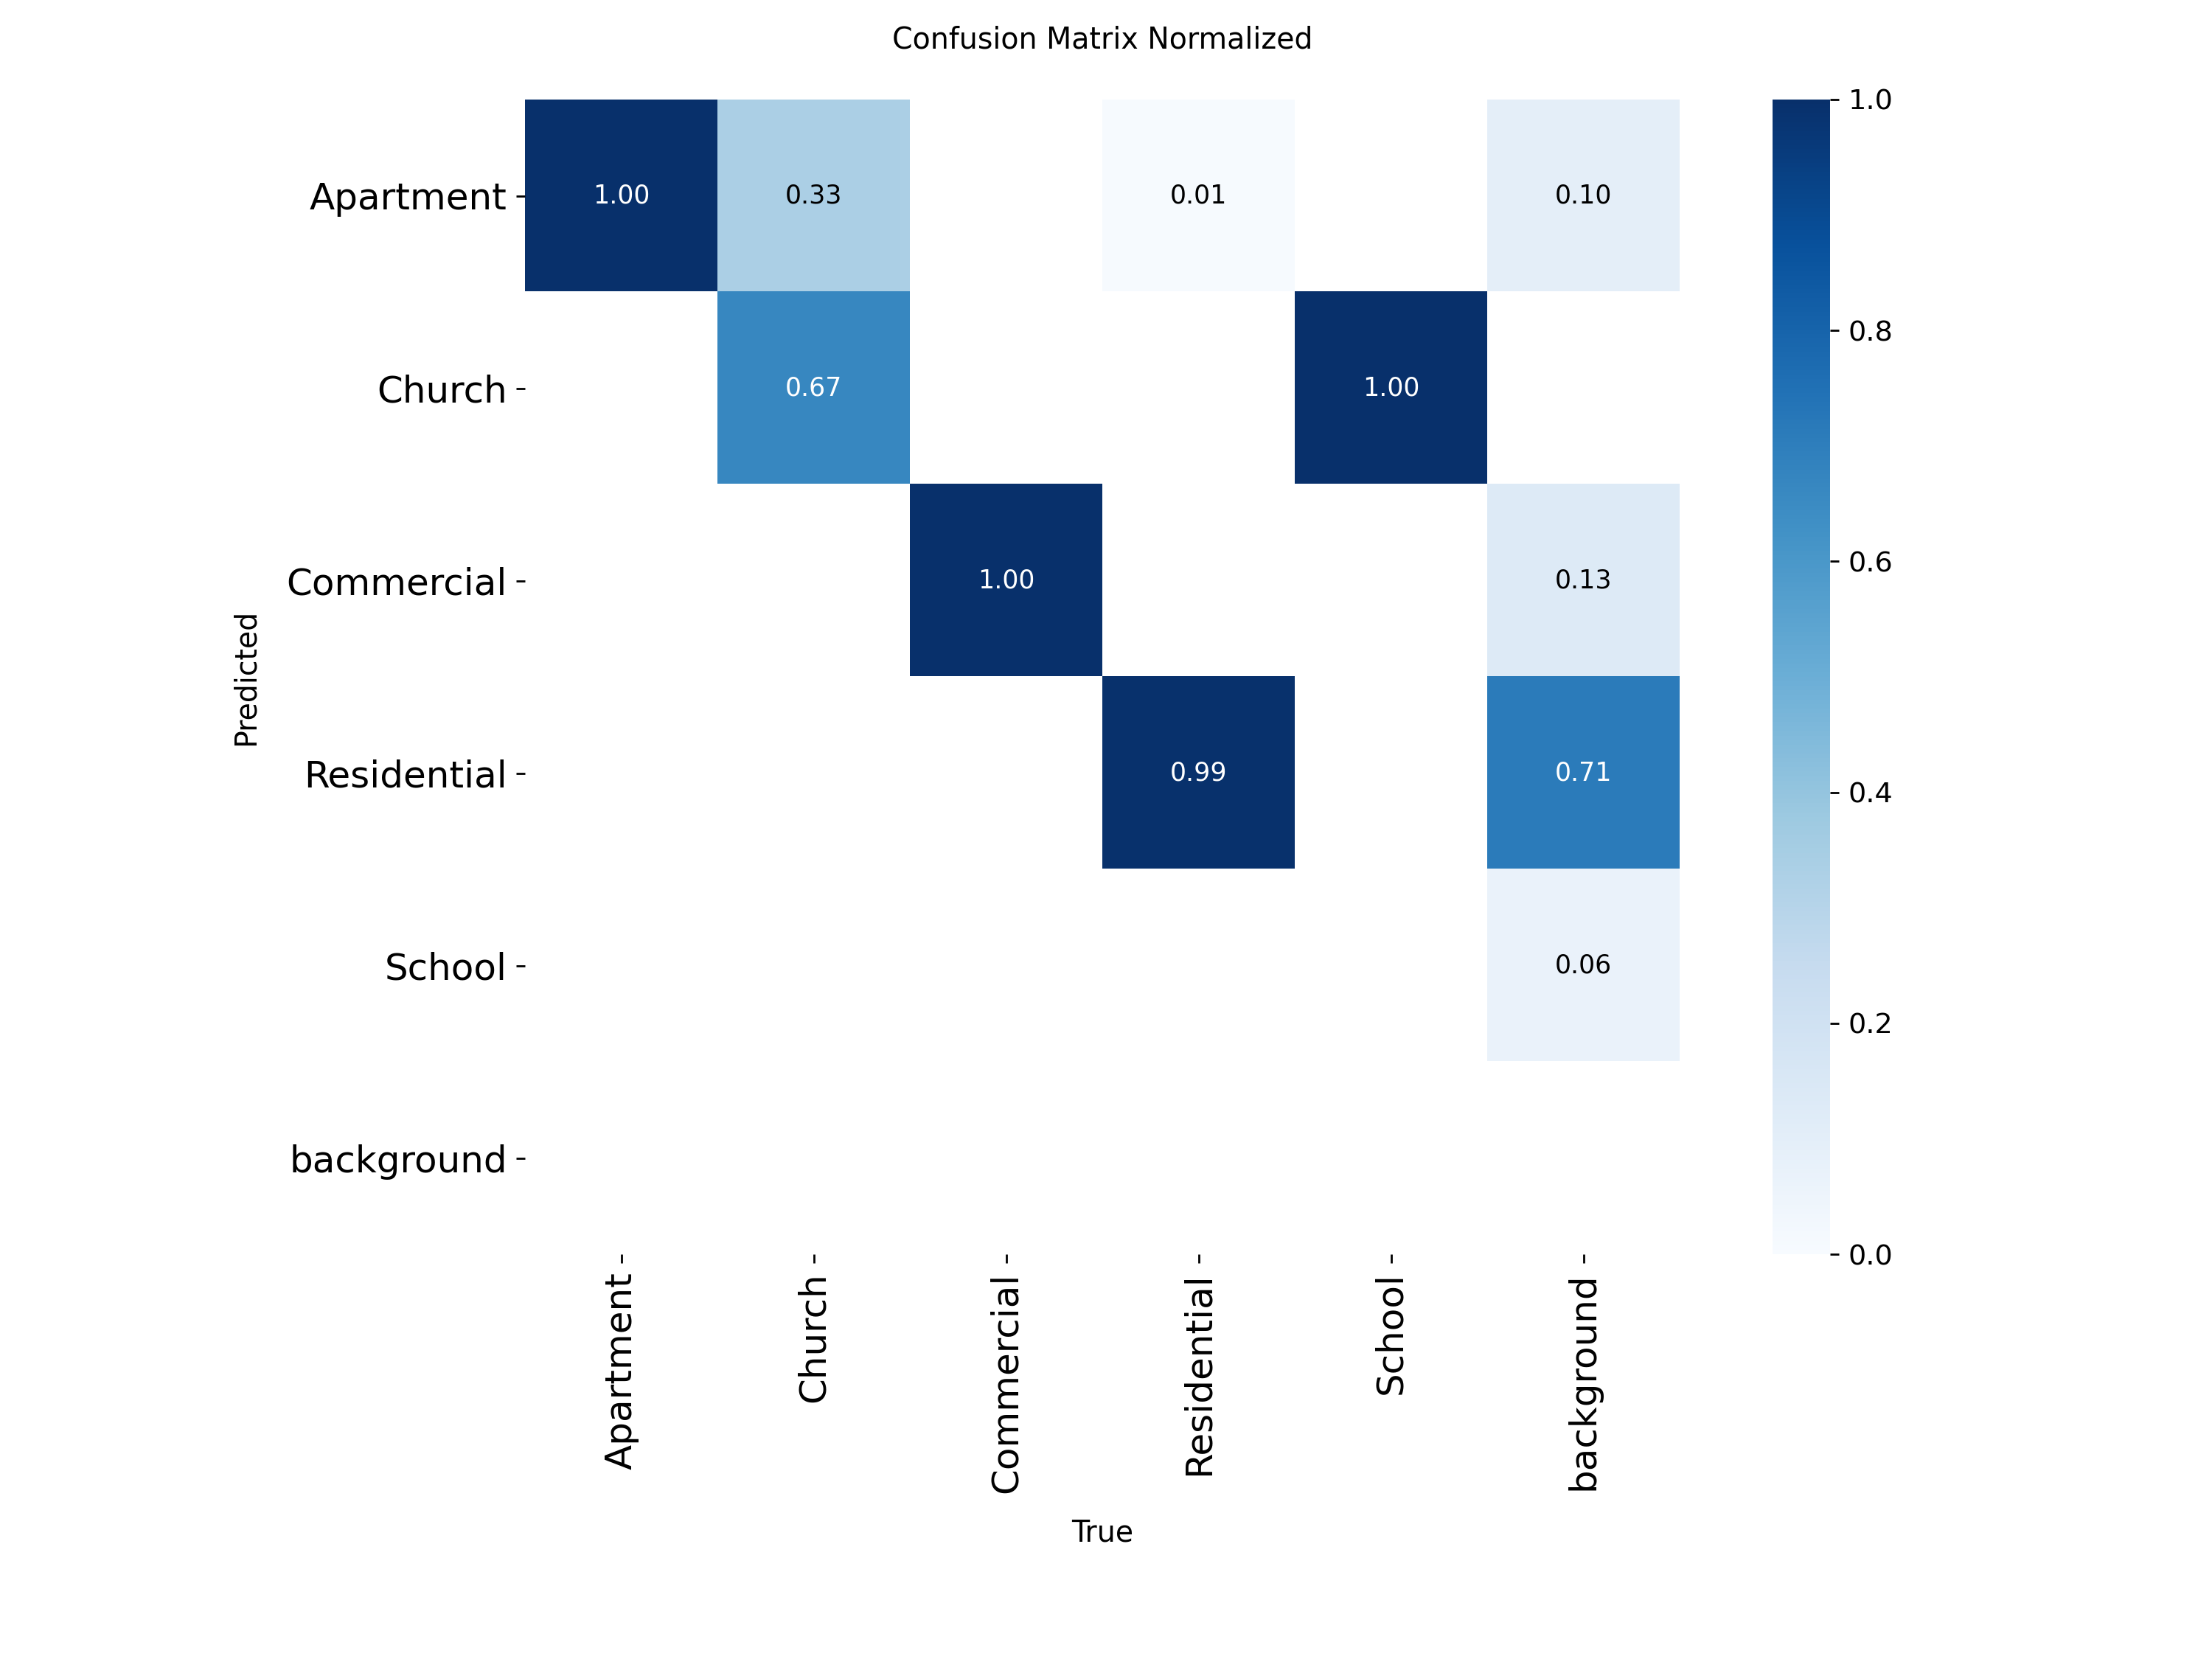
\includegraphics[width=1\linewidth,height=\textheight,keepaspectratio]{../runs/detect/logan_validation/confusion_matrix_normalized.png}

}

\subcaption{\label{fig-logan_cm_n}Logan Utah}

\end{minipage}%

\caption{\label{fig-confusion-matrix-val-cities}Normalized YOLO
confusion matrixes}

\end{figure*}%

\section{Conclusion and Future
Research}\label{conclusion-and-future-research}

The conclusion goes here.

As discussed by Hall et al., there are potential ethical problems with
such data collection. It strattles the line between public and private
information. This will need to be considered as further reserach is done
into this area as to stay on the right side of the
law.\autocite{hall_use_2021}

What does the future research look like?

Training models to detect other things such as cars, swing sets, patios,
etc.

Creating the process to predict household types based off the collected
data

Incorperating drone aerial imagery and extracing building footprints
from that.

Research into other remote sensing data and how it could be
incorperated.

\section{Acknowledgment}\label{acknowledgment}

The authors would like to thank\ldots{}

\printbibliography[title=References]

\end{document}

